\documentclass[11pt]{article}

\usepackage[review]{acl}

\usepackage{times}
\usepackage{latexsym}
\usepackage[T1]{fontenc}
\usepackage[utf8]{inputenc}
\usepackage{microtype}
\usepackage{inconsolata}
\usepackage{amssymb}

\usepackage{graphicx}
\usepackage{booktabs}
\usepackage{array}
\usepackage{enumitem}
\usepackage{xspace}
\usepackage{float}
\usepackage{xcolor}
\usepackage{xurl}
\usepackage{amsmath}
\usepackage{comment}
\usepackage{multirow}

\usepackage{pgfplots}
\pgfplotsset{compat=1.18}

% Packages for custom prompt boxes
\usepackage{tcolorbox}
\tcbuselibrary{breakable}

% Defining the PromptBlock environment
\newtcolorbox{PromptBlock}{
    colback=gray!5!white,      % Light gray background
    colframe=gray!50!black,    % Darker gray border
    boxrule=0.5pt,             % Thin, clean border line
    arc=2pt,                   % Slightly rounded corners
    left=6pt, right=6pt,       % Side padding
    top=6pt, bottom=6pt,       % Top/bottom padding
    fontupper=\small\ttfamily, % Makes the prompt text smaller and typewriter font (optional, remove \ttfamily if you want standard font)
    breakable                  % CRITICAL: Allows the box to split across pages
}

%\title{Evaluating LLM Pragmatic Competence via Colloquial Malay Pragmatic Particles}
\title{Can Large Language Models Handle Discourse Particles?\\A Case Study of Colloquial Malay}

\author{
  [Author 1 Name] \\
  [Affiliation 1] \\
  [email1@example.com]
  \And
  [Author 2 Name] \\
  [Affiliation 2] \\
  [email2@example.com]
  \AND
  [Author 3 Name] \\
  [Affiliation 3] \\
  [email3@example.com]
}

\begin{document}
\maketitle

\begin{abstract}
Discourse particles, such as \textit{well} and \textit{kind of}, are crucial components that enable LLMs to "speak" more like humans. They are used to convey emotions, intentions, and interpersonal meanings.
%, making them important for endowing Large Language Models (LLMs) with more human-like communicative competence.
However, existing studies have not yet built a comprehensive understanding of LLMs’ capabilities in handling discourse particles. The limited number of research focuses primarily on high-resource languages such as English. 
In this paper, we (1) propose \textsc{MalayPrag}, a benchmark designed to systematically evaluate and analyze LLMs’ capabilities in handling discourse particles in colloquial Malay; (2) introduce five attributes that provide a linguistically-grounded, unified framework for interpreting pragmatic functions of discourse particles. 
Applying these two, we prompt ten off-the-shelf LLMs to perform three predication tasks. 
%enabling us to investigate how LLMs handle discourse particles through the lens of their pragmatic functions.
The experimental results reveal substantial challenges for current LLMs to accurately connect between discourse particles and their pragmatic functions in Malay. The provision of the five attributes designed in this study is found to significantly improve the connections,  highlighting the need for structured scaffolding for models' pragmatic competence.
\textit{Our benchmark can be accessed via the link\footnote{https://anonymous.4open.science/r/MalayPrag-A285/README.md}}.
\end{abstract}

\section{Introduction}
%While Large Language Models (LLMs) are known to have pragmatic gaps in interpreting meanings that language use creates in context~\cite{liu2025pragmatic}, recent studies have endeavoured to develop pragmatics-tasked datasets and benchmarks to bridge these gaps \citep{sravanthi2024pub,ruis2023large,cong2024manner}. However, these efforts have primarily focused on English and other resource-rich languages, leaving low-resourced Southeast Asian languages largely untested \citep{ma2025pragmatics}.

%With the increasing need for LLMs to speak more like humans---for instance, with hesitations, uncertainty, and nuanced sentiments---discourse particles and their functions have attracted a considerable volume of interdisciplinary research \citep{sheffield2025just,sadlierbrown2024context,wang2025zeroshot,rocha2025crossgenre,eindor2022fortunately}.
As the demand for more \textit{human-like} communication in Large Language Models (LLMs) continues to grow, there is increasing interest in enabling LLMs to express phenomena such as hesitation, uncertainty, and nuanced sentiments. 
Consequently, discourse particles and their pragmatic functions\footnote{In linguistics, pragmatic function refers to the communicative role or purpose that a linguistic expression serves in a particular context, especially in relation to speakers’ intentions, social interaction, discourse structure, and inferred meaning.} have emerged as an increasingly important research topic~\citep{sheffield2025just,sadlierbrown2024context,wang2025zeroshot,rocha2025crossgenre,eindor2022fortunately}.
Discourse particles are unbound morphemes that encode implicit interpersonal dynamics, signaling multiple aspects of a speaker's intentions \citep{grzech2021discourse}. 
Typical examples of English particles include \textit{well}, \textit{like}, and \textit{kind of}. They do not contribute to the literal meanings of an utterance but are, nevertheless, important in organization (e.g., pause, turn-taking) and meaning negotiations (e.g., mitigation, politeness). In addition, they index identities, regions, genders, and other social qualities ~\citep{schiffrin1987discourse,fraser1999discourse}.
\begin{figure*}[t]
    \centering
    
\includegraphics[width=0.9\textwidth]{latex/figure1.png}
    \caption{Five-dimensional annotation schema for Malay discourse particle utterances. An utterance is evaluated by a native Malay speaker according to each of the five dimensions and the most appropriate attribute is assigned to the utterance capturing the speaker's intentions and the utterance's syntax. The linguistic theoretical basis for each attribute is available in the Appendix~\ref{tab:flattened-pragmatic-codebook}. Overall, the schema operationalizes pragmatic meaning as structured attributes that can be directly evaluated in LLM experiments.}
    \label{fig:details-of-annotations}
\end{figure*}

Understanding the capabilities and mechanisms of LLMs in handling discourse particles is essential for the development of more human-like language models given the well-known pragmatic gaps in LLMs when interpreting meanings that arise through language use in context~\cite{liu2025pragmatic}. 
Recent studies have sought to bridge these gaps by developing pragmatics-oriented datasets and benchmarks \citep{sravanthi2024pub,ruis2023large,cong2024manner}. 
However, these efforts have primarily focused on English and other high-resource languages, leaving low-resource Southeast Asian languages largely unexplored \citep{ma2025pragmatics}. 
To date, no prior work has investigated LLMs' understanding of discourse particles in Malay or its neighboring languages, despite their rich systems of discourse particles.

%Traditionally, the pragmatic functions of discourse particles have been studied through inductive corpus linguistics ~\citep{schiffrin1987discourse,fraser1999discourse,defelice2013classification, bunt2012iso}. While helpful for human linguistic theory, this human-centric approach creates a fundamental bottleneck for LLMs. 
%LLMs operate as statistical pattern matchers and struggle to map fuzzy, high-level pragmatic labels to actual syntax \citep{ruis2023large}. 
%To rigorously evaluate LLM pragmatic competence, invisible social intents must therefore be decomposed into discrete, computable attributes ~\citep{hovy2021importance,choi2023llms}, flattening subjective nuance into a structured feature matrix that a neural network can directly process.


In the meanwhile, LLMs have been found to struggle to capture pragmatic functions of discourse particles \cite{sheffield2025just}, as each discourse particle tends to have an excessive range of functions that vary by context, for example, the phrase "how-to-say" in Chinese alone has 15 different functions \cite{chen_functions_2023}. 
%it requires assessing how LLMs manipulate their pragmatic functions}.
%Traditionally, the pragmatic functions of discourse particles have been studied through inductive corpus linguistics ~\citep{schiffrin1987discourse,fraser1999discourse,defelice2013classification, bunt2012iso}. While helpful for human linguistic theory,
%LLMs struggle to capture the fine-grained categories of pragmatic functions \cite{sheffield2025just}. 
%map broad, abstract pragmatic labels to actual syntactic forms \citep{ruis2023large}. 
A potential solution to this issue is to explore the first-order epistemic, emotional, and linguistic attributes that underlie the varied pragmatic functions, hence translating the abstract notions of functions into discrete, computable variables~\citep{hovy2021importance,choi2023llms}. However, to the best of the authors' knowledge, the solution has not yet been experimentally examined. 
%Additionally, a singular discourse particle may vary in function (e.g.~\citet{SVENNEVIG202585} show that ``hello'' has 18 pragmatic functions). Therefore, we need a unified framework that underlies these pragmatic functions to bridge LLM comprehension.

In this paper, we not only present a new Colloquial Malay dataset of discourse particles (\textsc{MalayPrag}), but also develop five attributes for evaluating their pragmatic functions in context. The attribute design is grounded solidly on linguistic theories.
Figure~\ref{fig:details-of-annotations} demonstrates the five attributes (\textit{Epistemic Stance}, \textit{Listener Agreement}, \textit{Emotion}, \textit{Question Type}, and \textit{Particle Position}), and their classes for annotation. 
%that underlie pragmatic functions of Malay discourse particles.
%and that play an essential role for LLMs to reason interactional meanings in Malay. 
%These five attributes form a unified framework, decomposing abstract pragmatic labels to generalizable attributes, facilitating more precise evaluation of LLMs in handling discourse particles.

We apply the dataset and attributes to two Malay discourse particles, \textit{kan} and \textit{ke} (commonly spelled as \textit{ka} or \textit{kah}), because they provide a theoretically meaningful contrast in their pragmatic functions (see Section 2 for their details). We conduct two types of tasks to assess LLMs’ capabilities of handling Malay discourse particles: discourse particle interpretation and generation, measured by model accuracy. We test ten off-the-shelf LLMs.


The experimental results show that \textbf{(1)} LLMs exhibit substantial difficulty in interpreting the pragmatic functions of Malay discourse particles and \textbf{(2)} performance improves when the five attributes are provided (Figure~\ref{fig:details-of-annotations}). Accordingly, the contributions of this study are threefold:
\begin{enumerate}[leftmargin=*, itemsep=0pt, topsep=0pt]
    \item \textit{MalayPrag: A Novel Low-Resource Benchmark.} We introduce a rigorously verified dataset for Colloquial Malay pragmatics, addressing the critical lack of Southeast Asian representation in LLM evaluation.
    \item \textit{A Theory-Grounded, generalisable framework of five attributes for understanding discourse particle.} We propose five attributes as a unified framework that can be generalised for LLMs to learn pragmatic functions of discourse particles in Southeast Asian languages. \textit{To the best of our knowledge, this is the first attribute framework that enables the unified modeling of pragmatic functions in real-world data.} Note that \textit{kan} and \textit{ke} are also used in Indonesian. The attribute-based design also reduces annotator bias and standardizes subjective pragmatic interpretation for computational modeling.
    \item \textit{A fine-grained and comprehensive understanding of LLMs' capability of handling discourse particles.} We provide a detailed comparison of how general-purpose and Southeast Asia-focused LLMs perform on Malay discourse particles. This allows us to identify not only whether models fail, but where they fail. Our results show that LLMs' pragmatic competence in low-resource Southeast Asian languages is uneven, attribute-sensitive, and can be improved by explicit pragmatic scaffolding.
\end{enumerate}


%This suggests that LLMs are not entirely insensitive to pragmatic information, but their pragmatic reasoning is highly dependent on provided structure. Rather than resolving the problem, the improvement demonstrates the value of explicit pragmatic scaffolding and highlights the need for evaluation methods that can diagnose which components of pragmatic competence that models struggle with. 
%While both particles can occur in confirmation-oriented contexts, they differ in that \textit{kan} often tends towards agreement or alignment, whereas \textit{ke} more strongly indexes questioning or uncertainty.
%\textit{This contrast allows us to test whether LLMs can distinguish fine-grained pragmatic meanings that are not reducible to lexical items or syntax alone}.

%We evaluate seven state-of-the-art general-purpose models and two Southeast Asia-focused models to examine both broad multilingual performance and regionally specialized model behavior.
%(GPT-5, GPT-5.4 mini, Claude Sonnet 4.6, Claude Haiku 4.5, Gemini 3.1 Pro Preview, Gemini 3.1 Flash Lite, DeepSeek-v4-Pro, DeepSeek-v4-Flash, Llama-SEA-LION-v3.5-70B-R, and Gemma-SEA-LION-v4-27B-IT).
%Our dataset \textsc{MalayPrag} and evaluation metrics address this gap. By testing them on nine models,
%to evaluate their ability to process discourse particles. These tasks enable us to examine how LLMs understand and manipulate the pragmatic functions of discourse particles.
%\textbf{(1) Discourse Particle Interpretation:} This task evaluates a model's ability to decode the implicit social and interactional dynamics embedded within an utterance. This diagnostic isolates the model's raw cultural perception from its logical reasoning architecture. A model’s performance on this task demonstrates whether it can organically retrieve and comprehend the unspoken, context-dependent social realities established by a speaker, or if its comprehension is strictly limited to surface-level propositional semantics.
%\textbf{(2) Discourse Particle Generation:} This task assesses the model's ability to actively deploy contextually appropriate discourse particles within a masked language modeling paradigm. While interpretation tests passive comprehension, generation tests active, rule-bound execution. Performance on this task reveals whether an LLM can successfully fuse abstract meta-linguistic constraints (e.g., a mandate to express an "uncertain stance") with local syntactic probabilities. Success here proves that the model possesses true functional competence, capable of aligning its generative output with complex, culturally specific social intents rather than simply defaulting to statistical word-frequency biases.

%To obtain a comprehensive understanding of LLMs’ capabilities in handling Malay discourse particles, we design two types of tasks: discourse particle interpretation and generation, measuring LLMs on accuracy. We conduct evaluations on ten off-the-shelf LLMs.
%The experimental results show that \textbf{(1)} LLMs exhibit substantial difficulty in interpreting the pragmatic functions of Malay discourse particles and \textbf{(2)} performance improves when the task is decomposed by providing the attributes of our schema (Figure~\ref{fig:details-of-annotations}). 
%This suggests that LLMs are not entirely insensitive to pragmatic information, but their pragmatic reasoning is highly dependent on provided structure. Rather than resolving the problem, the improvement demonstrates the value of explicit pragmatic scaffolding and highlights the need for evaluation methods that can diagnose which components of pragmatic competence that models struggle with. 
%Our contributions are thus threefold:


\begin{comment}
Our contributions are thus threefold:

\begin{enumerate}[leftmargin=*]
    \item \textit{MalayPrag: A Novel Low-Resource Benchmark.} We introduce a rigorously verified dataset for Colloquial Malay pragmatics, addressing the critical lack of Southeast Asian representation in LLM evaluation.
    \item \textit{A Theory-Grounded Evaluation Schema.} We propose five attributes as evaluation metrics for pragmatic functions of Malay discourse particles. The attribute-based design reduces annotator bias and standardizes subjective pragmatic interpretation for computational modeling.
    \item \textit{A fine-grained and comprehensive understanding of LLMs' performance in dealing with discourse particles.} We provide a detailed comparison of how general-purpose and Southeast Asia-focused LLMs perform on Malay discourse particles across multiple pragmatic attributes, including epistemic stance, listener agreement, emotion, question type, and particle position. This allows us to identify not only whether models fail, but where they fail. Our results show that pragmatic competence in LLMs is uneven, attribute-sensitive, and improved but not solved by explicit pragmatic scaffolding.
\end{enumerate}
\end{comment}
%\textbf{Potential to generalise across Southeast Asian languages} 
%In addition, colloquial discourse particles are prevalent in Southeast Asian languages due to intensive language contact and immigration in the region. For example, \textit{kan} and \textit{ke} investigated in this paper are also used in Indonesian. Therefore, our design of evaluation metrics has the potential to be generalized across a variety of discourse particles in different Southeast Asian languages. 
    
    %We implement a two-part evaluation framework (diagnostic parsing and constrained generation) that isolates an LLM's logical reasoning capacity from its raw cultural perception.


\section{Related Work}

% Discourse particles are interactional devices used to manage common ground and project epistemic authority \citep{grzech2021discourse}. 

In Malay, \textit{kan} and \textit{ke} encode interactional meanings beyond propositional content. \textit{Kan} marks conjoint knowledge or requests listener agreement \citep{tay2016discourse,wouk1998solidarity}, as in ``Dia dah makan, \textbf{kan}?'' (`He already ate, right?'), while \textit{ke} marks interrogativity, uncertainty, confirmation-seeking, or rhetorical challenge, as in ``Awak marah \textbf{ke}?'' (`Are you mad?'). Since these particles vary across epistemic, interpersonal, affective, structural, and positional dimensions, we operationalize their pragmatic meanings through five computationally measurable attributes: \textit{Epistemic Stance}, \textit{Listener Agreement}, \textit{Emotion}, \textit{Question Type}, and \textit{Particle Position}. These attributes capture complementary dimensions of pragmatic particle meaning: common ground and listener orientation motivate \textit{Listener Agreement} \citep{wouk1998solidarity,stalnaker2002common}; epistemic stance and speaker authority motivate \textit{Epistemic Stance} \citep{karkkainen2003epistemic,grzech2021discourse}; and work on affective meaning motivates \textit{Emotion} as a cue to speaker attitude in interaction \citep{caffi1994pragmatics,buechel-hahn-2017-emobank}. Table~\ref{tab:flattened-pragmatic-codebook} summarizes the attribute settings, with full definitions in Appendix~\ref{app:codebook}.

% %original version
% In Malay, \textit{kan} operates as an addressee-oriented solidarity-building device that marks conjoint knowledge, establishing that information is shared or explicitly requesting listener agreement \citep{tay2016discourse,wouk1998solidarity}. For example, in the utterance ``Dia dah makan, \textbf{kan}?'' (`He already ate, right?'), the particle appears at the end of a declarative statement, transforming it into a confirmation-seeking question. Conversely, \textit{ke} turns declaratives into interrogatives and encodes uncertainty, confirmation-seeking, or rhetorical challenge, such as in ``Awak marah \textbf{ke}?'' (`Are you mad?'). Both particles frequently interact with various question types, ranging from genuine yes/no interrogatives to rhetorical challenges, and particle positions. 

% % They mostly occupy the middle or sentence-final positions, but can also appear at the beginning of sentences, as in ``\textbf{Kan} saya dah cakap?'' (`Didn't I tell you?' / `I told you so, didn't I?'), which emphasizes the speaker's epistemic authority by framing the proposition as pre-established knowledge that the listener is expected to concede to.

% To capture this range of interactional meanings systematically, we operationalize pragmatic particle meaning through five computationally measurable attributes: \textit{Epistemic Stance}, \textit{Listener Agreement}, \textit{Emotion}, \textit{Question Type}, and \textit{Particle Position}. These attributes draw on prior work on common ground, listener orientation, epistemic stance, speaker authority, and affective meaning in pragmatic and computational language understanding \citep{wouk1998solidarity,stalnaker2002common,karkkainen2003epistemic,grzech2021discourse,caffi1994pragmatics,buechel-hahn-2017-emobank}. Table 6 summarizes the attribute settings, with full definitions in Appendix A.

% Original Explanation of Theoretical Foundations of Annotation Schema 
% Drawing on \citet{wouk1998solidarity} and \citet{stalnaker2002common}, we operationalized the attribute \textit{Listener Agreement} to capture common ground and the speaker's expectation of a response, as indicated by the particles. Concurrently, \textit{Epistemic Stance} was derived from \citet{karkkainen2003epistemic} and \citet{grzech2021discourse} to capture the speaker's degree of certainty and authority over the information presented. To capture the affective dimension of particle use, we include \textit{Emotion} as an annotation attribute. Since online text lacks prosodic cues such as intonation, stress, and pitch, affective stance must be inferred from textual and paralinguistic cues, including punctuation, capitalization, emojis, lexical choice, and discourse context. This follows work linking pragmatic competence to speaker attitudes and affective meanings in interaction (Caffi and Janney, 1994), as well as NLP work that operationalizes emotion labels as a measurable dimension of affective language understanding (Buechel and Hahn, 2017). Following the aforementioned linguistic findings, we translated these abstract theories into the five discrete, computationally measurable attributes: Epistemic Stance, Listener Agreement, Emotion, Question Type, and Particle Position. Table 6 summarizes the setting of these attributes. Their definitions are included in Appendix A.

Previous studies have found that LLMs struggle to interpret pragmatic functions of discourse particles ~\citep{sheffield2025just,sadlierbrown2024context,eindor2022fortunately}. For example, \citet{sheffield2025just} demonstrate that LLMs fail to distinguish the overlapping senses of the English particle \textit{just}; moreover, providing surrounding conversational context actively decreases model accuracy rather than aiding disambiguation.

However, it is worth noting that the aforementioned studies primarily used direct, coarse-grained classifications of pragmatic functions, with the hope that LLMs would learn the association between language data and annotated functions automatically. This approach, however, results in severe limitations, including low inter-rater reliability (IRR), data sparseness \citep{defelice2013classification}, and models failing to grasp the underlying reasons why a particle was used. Our approach innovatively bridges the use of discourse particles and their pragmatic functions via the five attributes, by which LLMs' performance improves.

%Computationally, unsupervised clustering algorithms such as K-Means have successfully grouped noisy, unlabeled dialogue to discover underlying user intents \citep{park2024analysis}. Notably, \citet{foo2024disentangling} demonstrated that clustering isolated utterance embeddings effectively disentangles the macro-functions of highly polysemous Singlish discourse particles (e.g., \textit{lah}, \textit{meh}). This offers a direct computational precedent for our approach: utilizing underlying variables to infer macro-pragmatic functions, yielding a more accurate and scientifically valid evaluation of LLM competence.

\section{Methodology}
%\begin{figure}[t]
    %\centering
    %
\includegraphics[width=0.5\textwidth]{latex/figure2.png}
    %\caption{Overarching benchmarking pipeline.}
    %\label{fig:overarching-benchmarking-pipeline}
%\end{figure}

\begin{figure}[t]
\centering
\small
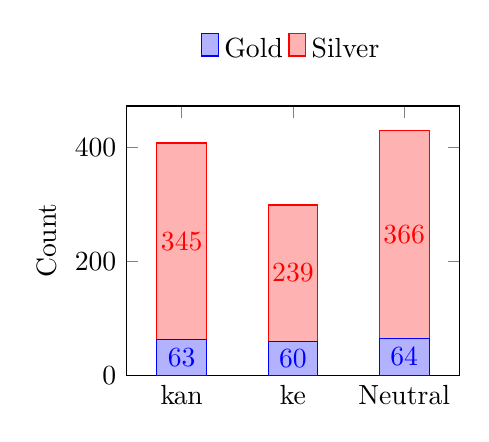
\begin{tikzpicture}
\begin{axis}[
    ybar stacked,
    bar width=18pt,
    width=0.48\textwidth,
    height=5cm,
    ymin=0,
    ylabel={Count},
    symbolic x coords={kan, ke, Neutral},
    xtick=data,
    legend style={
        at={(0.5,1.12)},
        anchor=south,
        legend columns=2,
        draw=none
    },
    nodes near coords,
    enlarge x limits=0.25,
]
\addplot coordinates {(kan,63) (ke,60) (Neutral,64)};
\addplot coordinates {(kan,345) (ke,239) (Neutral,366)};

\legend{Gold, Silver}
\end{axis}
\end{tikzpicture}

\caption{
Distribution of Gold and Silver annotation splits across \textit{kan}, \textit{ke}, and neutral baseline utterances.
Overall, the splits maintain a balanced coverage of particle and neutral cases for both adjudicated evaluation and broader analysis.
}
\label{fig:dataset-distribution}
\end{figure}

This section details the construction of the \textsc{MalayPrag} dataset. We first outline the data collection and filtering process. Next, we describe the translation of linguistic theory into our annotation schema. Afterwards, we introduce how pragmatic functions were extracted from the data, and 
%Finally, we detail the human annotation process and justifications for our Gold/Silver dataset split \textcolor{red}{GL: why we need to highlight the gold and silver dataset split?}, followed by the LLM evaluation pipeline.
finally we elaborate the tasks that can be leveraged to understand LLMs' capabilities in handling discourse particles.

\subsection{Data collection}
 Data was sourced from naturally occurring informal Malay utterances on Reddit and Twitter/X containing the particles \textit{kan} and \textit{ke}. To augment the dataset, we synthesised a sample of \textit{kan} sentences to create (1) neutral sentences (by removing \textit{kan}) and substituted utterances (replacing \textit{kan} with \textit{ke}). All synthesised sentences were validated by native speakers to ensure naturalness. The neutral sentences are used to test whether LLMs can distinguish the differences in pragmatic functions with/without the particle.

%Sentences were isolated from surrounding conversational threads to strictly replicate the text-only evaluation conditions encountered by LLMs. 
We used regular expressions to flag Indonesian phrasing, foreign-language interference, and prepositional uses of the homograph \textit{ke} (`to'), followed by manual inspection for final data cleaning.

A total of 1{,}137 data was labeled by native Malay-speaking linguists trained in pragmatic analysis. The final dataset was bifurcated into a GOLD and SILVER split for different modelling needs. The GOLD dataset ($N=187$) consists of utterances independently annotated by three annotators, with disagreements resolved via majority voting or lead-author adjudication. This set was used as the ground-truth for LLM evaluation. The SILVER dataset ($N=950$) comprises utterances labeled only by a single trained annotator, and it was used for the extraction of pragmatic functions. Figure \ref{fig:dataset-distribution} illustrates the data split.

%It provides the necessary statistical weight for K-Means intent induction clustering, actively leveraging the algorithm's inherent noise tolerance.
\begin{comment}
\begin{table*}[t]
\centering
\footnotesize
%\small
\renewcommand{\arraystretch}{1.15}
\setlength{\tabcolsep}{6pt}

\begin{tabular*}{\textwidth}{@{\extracolsep{\fill}} p{0.30\textwidth} p{0.70\textwidth}}
\toprule
\textbf{Category} & \textbf{Task Description} \\
\midrule

\multirow{3}{*}{\textbf{Task 1} Attribute/Function Prediction}
& (1a) Attribute prediction \\

& (1b) Pragmatic function prediction \textbf{without} attribute provision \\

& (1c) Pragmatic function prediction \textbf{with} attribute provision \\
\midrule

\multirow{4}{*}{\textbf{Task 2} Discourse Particle Predication}
& (2a) Particle predication from raw data \\

& (2b) Particle predication with attributes provided \\

& (2c) Particle predication with pragmatic functions provided \\

& (2d) Particle predication with both attributes and pragmatic functions provided \\
\midrule

\multirow{2}{*}{\textbf{Ablation Experiment}}
& (3a) Pragmatic function prediction via CoT \\

& (3b) Particle predication with pragmatic functions and CoT provided \\
\bottomrule
\end{tabular*}
\label{tab:evaluation_tasks}
\caption{Evaluation tasks}
\end{table*}
\end{comment}



\subsection{Attribute annotation}
Most existing discourse annotation schemes are tailored to English and high-resource languages, making direct porting ineffective for low-resource languages \citep{vargas2025discourse}. Furthermore, applying generic categories without explicit, well-documented definitions leads to subjective bias and high annotator disagreement \citep{crible2015unified}. Therefore, we develop our annotation schemes based on existing linguistic research of Southeast Asian discourse particles and commonly agreed empirical findings across languages. Details can be found in Appendix \ref{app:codebook}
%Table 1 presents the annotation schemes of the five attributes and their taxonomy as well as the theoretical backbones.



To be specific, within \textit{Epistemic Stance}, there are three options: Certain, Uncertain, and Neutral. A \textit{Certain} classification denotes that the speaker holds full epistemic authority, presenting the proposition as factual or unquestionable, whereas \textit{Uncertain} reflects speculation, doubt, or an active hypothesis. For \textit{Listener Agreement}, \textit{Assumed Agreement} dictates that the proposition is framed as pre-existing common ground; the speaker expects the listener to simply align or concede, treating the utterance as a rhetorical check rather than a genuine inquiry. Conversely, \textit{Confirmation Seeking} indicates a genuine request for verification where the speaker actively leaves room for the listener to contest, correct, or reject the premise. In contrast, structurally objective variables such as \textit{Particle Position} (\textit{Front, Middle/End, N/A}) and \textit{Question Type} were strictly defined by their syntactic markers and require minimal interpretation.


\subsection{Extracting pragmatic functions from attribute clustering}
As emphasized above, we do not directly annotate pragmatic functions for LLMs to interpret, which has been evidenced to be ineffective in previous studies \citep{defelice2013classification}. Instead, we used the five attributes annotated to obtain pragmatic functions. Specifically, we cluster the annotated attributes using K-means on both GOLD ($N=187$) and SILVER ($N=950$) datasets (total $N=1{,}137$). The reason for both datasets to be involved in this process is to take into account both collective understanding of the discourse particles -- that are represented by the agreements in GOLD dataset -- and individual variations represented by the SILVER dataset. 


%To uncover the latent, context-dependent macro-functions of the target discourse particles without imposing top-down English-centric biases, 
%we employed an unsupervised intent induction pipeline. K-Means clustering was applied to the combined GOLD ($N=187$) and SILVER ($N=950$) datasets (total $N=1{,}137$) to maximize the statistical density of the vector space while leveraging the algorithm's natural noise tolerance. Utterances were vectorized using the [CS TEAM: INSERT EXACT EMBEDDING MODEL HERE, e.g., \texttt{paraphrase-multilingual-mpnet-base-v2}] embedding model to capture deep semantic and syntactic relationships.

Spatially close clusters of the attributes are expected to represent the same or similar pragmatic functions of a discourse particle, while distanced clusters represent distinctive pragmatic functions. We should emphasise that the clustering results do not reveal the pragmatic functions automatically. Rather, following the K=16 clustering, human linguists conducted a qualitative review of the utterances within the 16 clusters to inductively assign discrete, overarching ``pragmatic function'' labels, thereby establishing a data-driven taxonomy for the subsequent evaluations of LLMs.



 To illustrate the correlations between pragmatic functions and clustering of five attributes, for example, the pragmatic function ''Information-seeking verification'' is often represented by the cluster that contains an uncertain epistemic stance, a confirmation-seeking listener agreement, neutral emotion, and an interrogative structure. This specific constellation of attributes indicates that the discourse particle (predominantly \textit{ke}) is functioning as a genuine request for clarification where the speaker actively leaves room for disagreement. Conversely, the ''Negative rhetorical challenge'' function emerges from a sharply contrasting attribute pattern: a certain epistemic stance, assumed listener agreement, a rhetorical question structure, and strong negative affect. In this context, the underlying attributes dictate that the particle functions not as an inquiry, but as a discourse device to criticize, mock, or forcefully evaluate a proposition. Appendix \ref{app:particle-functions} presents representative examples of these derived pragmatic functions.

%The algorithm was explicitly constrained to an initial hyperparameter limit of $K=16$ distinct clusters. 
%By mathematically grouping the utterances based on spatial proximity in the embedding space, the algorithm surfaced underlying structural patterns of particle usage. 


\begin{table}[t]
\centering
\footnotesize
\renewcommand{\arraystretch}{1.15}
\setlength{\tabcolsep}{2pt}

\begin{tabular}{llcc}
\toprule
\textbf{Prediction} & \textbf{Input} & \textbf{Prompting} & \textbf{+ CoT} \\
\midrule

\shortstack[l]{\textbf{T1} Attribute}
  & Raw data                    & \checkmark & \\
\midrule

\multirow{2}{*}{\shortstack[l]{\textbf{T2} Pragmatic\\Function}}
  & Raw data          & \checkmark & \checkmark \\
  &  + Attributes             & \checkmark & \\
\midrule

\multirow{4}{*}{\shortstack[l]{\textbf{T3} Particle}}
  & Raw data               & \checkmark & \\
  &  + Attributes             & \checkmark & \\
  & + Pragmatic functions    & \checkmark & \checkmark \\
  & + Attr.\ + prag.\ func.  & \checkmark & \\
\bottomrule
\end{tabular}

\caption{Evaluation tasks and conditions. Overall, the benchmark separates attribute prediction, pragmatic function prediction, and particle prediction to isolate where models succeed or fail.}
\label{tab:evaluation_tasks}
\end{table}



\subsection{Evaluation Tasks}
To systematically evaluate LLMs' capability to handle the pragmatics of Malay discourse particles, we conduct three evaluation tasks: attribute prediction, pragmatic function prediction, and discourse particle prediction. Table \ref{tab:evaluation_tasks} outlines each task and their conditions. 
%The pipeline consists of two distinct task categories designed to isolate latent structural logic from raw context extraction.

\paragraph{Task 1: Attribute Prediction.} 

%Task 1 allows us to distinguish between two sources of model failure: attribute-level failure and pragmatic function-mapping failure. If a model performs poorly on Test 1a, it suggests difficulty recognizing local pragmatic cues such as epistemic stance or listener agreement. If performance improves substantially in Test 1c, this suggests that the model can use explicit pragmatic information once provided, but struggles to infer it independently from colloquial Malay input. If performance remains poor even with gold attributes, this suggests a deeper failure to map pragmatic features onto discourse-particle functions.

%\textcolor{red}{Please do not use Task 1a to refer to attribute prediction, no reviewers can remember this. Also for other tasks, please use exactly their names like pragmatic function prediction w/o attributes. Keeping in mind that remembering how the pragmatic function can be predicted with or without attributes is already difficult for reviewers, they would be dead if we use encrypted language to refer to tasks.}

This task evaluates whether LLMs can predict the five attributes from raw data. 

\paragraph{Task 2: Pragmatic Function Prediction.} This task comprises three subtasks. In \textbf{(2a) Function prediction from raw data:} The model predicts predicts the overarching pragmatic function from the utterance alone. In \textbf{(2b) Function prediction via CoT:} The model predicts predicts pragmatic function given utterance and Chain-of-Thought (CoT) \citep{wei2022chain}. In \textbf{(2c) Function prediction via attributes:} The model predicts pragmatic functions given an utterance and its human-annotated attributes. Comparing the three subtasks allows us to confirm the effectiveness of attributes in bridging between discourse particles and their pragmatic functions, especially compared to CoT as a strong baseline.


% This task assesses LLMs' interpretations of the attributes and pragmatic functions of the discourse particles.
% It comprises three sub-tasks: 
% \textbf{(1a) Attribute Prediction} in which the model predicts the five discrete attributes from an utterance. If a model performs poorly on this test, it suggests difficulty recognizing local pragmatic cues such as epistemic stance or listener agreement.
% \textbf{(1b) Attribute-unprovided and (1c) Attribute-provided Function Prediction}, in which the model performs zero-shot prediction of the overarching pragmatic functions either from an utterance together with its underlying human-annotated attributes or solely from the utterance itself. 
% If performance is strong when given ground-truth attributes but poor without them, this suggests that the model can leverage explicit pragmatic information once provided but struggles to infer it independently from colloquial Malay input. 
% If performance remains poor even with ground-truth attributes, this indicates a deeper limitation in mapping pragmatic features to discourse-particle functions.
%and  Comparing Test 1b and Test 1c shows the effectiveness of our attributes in predicting pragmatic functions.

\paragraph{Task 3: Discourse Particle Prediction.} 

This task evaluates whether LLMs can select the appropriate particle, \textit{kan}, \textit{ke}, or neutral (no particle), for a masked utterance. 
%While Task 1 tests interpretation from particle form to pragmatic meaning, Task 2 tests the reverse mapping from pragmatic context to linguistic form. This is non-trivial because the same propositional content may require different particles depending on whether the speaker assumes agreement, seeks confirmation, or presents a neutral statement.
It includes five prompting conditions: \textbf{(3a) Particle prediction from raw data}, using only the masked utterance; \textbf{(3b) Attribute-provided prediction}, adding human-annotated attributes; \textbf{(3c) Function-provided prediction}, adding the target pragmatic function; \textbf{(3d) Particle prediction with attribute + function provided}, adding both; and \textbf{(3e) Particle prediction with CoT + function}, adding pragmatic functions with CoT prompts. Comparing these conditions tests whether explicit pragmatic scaffolding improves particle selection.
%distinguishing failures to infer pragmatic context from failures to map that context onto Malay particle forms.

% This task requires models to fill the discourse particle that has been masked in an utterance. 
% This task evaluates whether LLMs can select an appropriate Malay discourse particle to realize a given pragmatic context. While Task 1 tests interpretation, Task 2 tests the reverse mapping from pragmatic meaning to linguistic form. This is important because particles such as kan and ke are not interchangeable surface markers: the same propositional content may require kan, ke, or no particle depending on whether the speaker assumes agreement, seeks verification, or presents a neutral statement. Successful generation therefore indicates that a model can connect pragmatic meaning to particle choice, while failure reveals whether it over-relies on surface interrogative form, defaults to frequent particles, or fails to distinguish confirmation-oriented meanings from interrogative ones.
% It has three options: \textit{kan}, \textit{ke}, or a neutral blank. 

% We have four sub-tasks:
% \textbf{(2a) Unprovided Particle Generation} provides only the raw masked utterance for the models to fill the blank; \textbf{(2b) Attribute-provided Particle Generation} appends target human annotated attributes to the masked utterance; \textbf{(2c) Function-provided Particle Generation} appends a target pragmatic functions to assist LLMs to make the choice; and \textbf{(2d) Attribute \& Function-provided Particle Generation} is a combination of both (2b) and (2c). Comparing provided and unprovided settings allows us to test whether explicit pragmatic information helps models select the appropriate particle. If models improve under constrained prompting, this suggests that they can use explicit pragmatic cues but may not reliably infer them from raw utterance. If they do not improve, this suggests a deeper weakness in mapping pragmatic representations to Malay particle forms.

%\paragraph{Ablation Experiment: Chain of Thought (CoT) Baselines.} 
%We introduce Chain-of-Thought (CoT) \citep{wei2022chain} as a strong baseline to compare with our attribute-based approach in terms of effectiveness in predicting pragmatic functions and discourse particles.
%model failures stem from insufficient explicit reasoning or from missing pragmatic cues \citep{wei2022chain}. CoT prompts require models to reason step-by-step before producing a final answer, allowing comparison with our attribute-based scaffolding.
%\textbf{(3a) Pragmatic function prediction via CoT} predicts the overarching pragmatic function from the raw utterance alone after step-by-step reasoning. \textbf{(3b) Particle prediction with function + CoT provided} receives the masked utterance and target pragmatic function, then reason before selecting a particle. 
%We compare this with \textbf{(2d) Attribute-and-Function-Provided Particle Generation} to test whether models can map pragmatic function to particle form without explicit attributes.
%We compare this with both \textbf{(1b) Attribute-Unprovided Function Prediction} and \textbf{(1c) Attribute-Provided Function Prediction} to test whether CoT can recover the cues captured by the attribute framework. 

% To rigorously validate whether the models' failure in pragmatic deduction stems from a fundamental deficit in cultural perception rather than a mere lack of reasoning effort, we introduce two Chain-of-Thought (CoT) baselines. CoT prompting forces the model to articulate intermediate reasoning steps before arriving at a final output, effectively maximizing its latent logical capacity \citep{wei2022chain}. There are two sub-tasks: 
% (3a) CoT Attribute-unprovided Function Prediction mirrors (1b) Attribute-unprovided Function Prediction. Models are provided with the raw Colloquial Malay utterance and asked to predict the overarching pragmatic function. Crucially, the foundational attributes are withheld. Instead, the model is explicitly instructed to generate a step-by-step reasoning before outputting its final classification. By comparing this CoT baseline against both (1b) Attribute-unprovided and (1c) Attribute-provided Function Prediction, we isolate the exact nature of the LLM bottleneck: if CoT results in lower accuracy than when given our attribute framework, it supports that explicit structural scaffolding is required to compensate for a lack of internal cultural knowledge. (3b) CoT Function-provided Particle Generation mirrors (2c) Function-provided Particle Generation, serving as an ablation for Task 2. By comparing the results to (2d) Attribute \& Function-provided Particle Generation, we will be able to identify whether models can bridge social intent to syntactic form without being given the attributes.

\section{Experimental Setting and Results}
This section reports the experimental settings and empirical findings for the tasks above.

\paragraph{Models.} We evaluate ten off-the-shelf LLMs that span varying parameter scales, training paradigms, and regional specialisation. Eight are general-purpose frontier models accessed via their official APIs: GPT-5 and GPT-5.4-mini (OpenAI), Claude Sonnet 4.6 and Claude Haiku 4.5 (Anthropic), Gemini 3.1 Pro and Gemini 3.1 Flash (Google), and DeepSeek-v4-Pro and DeepSeek-v4-Flash (DeepSeek). To examine whether regional training affects pragmatic competence in Malay, we additionally include two open-weight Southeast Asia-focused models from the SEA-LION family~\citep{ng2025sea,koh2025mitigating}: Llama-SEA-LION-70B and Gemma-SEA-LION-27B. 

\paragraph{Evaluation data.} All tasks are conducted on the benchmark \textsc{MalayPrag} ($N=187$), in which every utterance has been independently annotated by three trained native Malay linguists, with disagreements resolved through majority voting or lead-author adjudication. 

\paragraph{Prompting and inference.} All tasks are run in a zero-shot setting, besides the CoT baselines in ablation experiments. 
% For Attribute Prediction task, each utterance is prompted twice, once in English and once in Malay, in order to probe the native prompting penalty in low-resource meta-linguistic reasoning. All remaining tasks  use English instructions, since the goal is to test the model's pragmatic interpretation of the Malay utterance rather than its meta-linguistic comprehension. 
To minimize sampling variance, we set temperature to $0$ (greedy decoding) for all models and constrain outputs to a single label from the closed set specified by each prompt template. The full prompting templates for every task are provided in Appendix~\ref{app:prompt_templates}.

\paragraph{Evaluation metric.} Following prior work on pragmatic benchmarking~\citep{sravanthi2024pub,sheffield2025just}, we report classification accuracy against the benchmark \textsc{MalayPrag}. For attribute prediction Task, accuracy is computed per attribute and then averaged across the five attributes. For pragmatic function prediction tasks, accuracy is computed over the seven pragmatic-function labels; for particle prediction Tasks, accuracy is computed over the three particle choices (\textit{kan}, \textit{ke}, neutral). The corresponding random-chance baselines are approximately $33\%$ or $50\%$ for attribute prediction, $14.3\%$ for pragmatic-function prediction, and $33.3\%$ for particle generation.

% \subsection{Experimental Setting}

% \textcolor{red}{GL: Bocheng, please complete this subsection.}
% We tested ten state-of-the-art language models across varying parameter sizes and training paradigms: GPT-5, GPT-5.4-mini, Claude Sonnet 4.6, Claude Haiku 4.5, Gemini 3.1 Pro, Gemini 3.1 Flash, DeepSeek-v4-Pro, DeepSeek-v4-Flash, Llama-SEA-LION-70B, and Gemma-SEA-LION-27B. To maintain strict scientific validity and prevent low inter-rater reliability from introducing label noise into evaluations, all tests were restricted exclusively to the fully adjudicated human GOLD dataset ($N=187$). 
%\subsection{Pragmatic Function Discovery}
%The unsupervised K-Means intent induction pipeline was initialized with a hyperparameter of $K=16$ distinct mathematical clusters. Following the spatial grouping of utterance embeddings, human linguists fluent in Colloquial Malay conducted a rigorous qualitative review of the sentences within each cluster to determine whether the mathematical boundaries correlated with observable linguistic patterns. Crucially, the qualitative analysis revealed that the algorithm did not cleanly partition the dataset based on overt surface forms; that is, it did not simply isolate all \textit{kan} instances from all \textit{ke} instances. Instead, the clusters formed cross-particle groupings driven by underlying pragmatic intentions and syntactic contexts, as demonstrated by the five attributes. Recognizing distinct pragmatic and semantic overlaps among the initial 16 mathematical partitions, the linguistic team inductively collapsed them into seven overarching qualitative pragmatic functions. Full descriptions of these pragmatic functions are provided in Appendix C.

\begin{table*}[t]
    \centering
    \tiny
    \setlength{\tabcolsep}{2pt}
    \resizebox{\textwidth}{!}{%
    \begin{tabular}{lcccccccccccc}
        \toprule
        \textbf{Model} & \multicolumn{2}{c}{\textbf{Epistemic}} & \multicolumn{2}{c}{\textbf{Agreement}} & \multicolumn{2}{c}{\textbf{Emotion}} & \multicolumn{2}{c}{\textbf{Question}} & \multicolumn{2}{c}{\textbf{Position}} & \multicolumn{2}{c}{\textbf{Overall Avg.}} \\
        \cmidrule(lr){2-3} \cmidrule(lr){4-5} \cmidrule(lr){6-7} \cmidrule(lr){8-9} \cmidrule(lr){10-11} \cmidrule(lr){12-13}
        & \textbf{EN} & \textbf{MS} & \textbf{EN} & \textbf{MS} & \textbf{EN} & \textbf{MS} & \textbf{EN} & \textbf{MS} & \textbf{EN} & \textbf{MS} & \textbf{EN} & \textbf{MS} \\
        \midrule
        GPT-5 & 0.706 & 0.765 & 0.594 & 0.524 & 0.797 & 0.738 & 0.695 & 0.711 & 0.901 & 0.884 & 0.742 & 0.724 \\
        GPT-5.4-mini & 0.583 & 0.449 & 0.631 & 0.519 & 0.797 & 0.770 & 0.604 & 0.626 & 0.752 & 0.777 & 0.700 & 0.628 \\
        Claude Sonnet 4.6 & 0.749 & 0.733 & 0.588 & 0.449 & 0.754 & 0.631 & 0.711 & 0.524 & 0.942 & 0.883 & 0.752 & 0.644 \\
        Claude Haiku 4.5 & 0.749 & 0.636 & 0.578 & 0.449 & 0.701 & 0.684 & 0.679 & 0.679 & 0.860 & 0.771 & 0.722 & 0.644 \\
        Gemini 3.1 Pro & 0.759 & 0.802 & 0.476 & 0.433 & 0.743 & 0.727 & 0.711 & 0.668 & 0.818 & 0.826 & 0.721 & 0.691 \\
        Gemini 3.1 Flash & 0.759 & 0.802 & 0.476 & 0.449 & 0.743 & 0.727 & 0.711 & 0.684 & 0.818 & 0.843 & 0.721 & 0.701 \\
        DeepSeek-v4-Pro & 0.615 & 0.668 & 0.465 & 0.476 & 0.749 & 0.727 & 0.695 & 0.674 & 0.942 & 0.934 & 0.696 & 0.696 \\
        DeepSeek-v4-Flash & 0.706 & 0.722 & 0.476 & 0.438 & 0.754 & 0.754 & 0.679 & 0.690 & 0.942 & 0.884 & 0.713 & 0.698 \\
        \midrule
        Llama-SEA-LION-70B & 0.348 & 0.433 & 0.278 & 0.433 & 0.540 & 0.369 & 0.406 & 0.417 & 0.868 & 0.554 & 0.499 & 0.441 \\
        Gemma-SEA-LION-27B & 0.717 & 0.679 & 0.524 & 0.529 & 0.690 & 0.711 & 0.615 & 0.599 & 0.612 & 0.722 & 0.660 & 0.648 \\
        \midrule
        \textbf{Average} & 0.669 & 0.669 & 0.509 & 0.470 & 0.727 & 0.684 & 0.651 & 0.627 & 0.845 & 0.808 & 0.693 & 0.652 \\
        \bottomrule
    \end{tabular}%
    }
    \caption{Attribute Prediction accuracy for English (EN) and Malay (MS) prompts. Overall, models perform unevenly across attributes, with position being the easiest attribute and listener agreement remaining the most challenging.}
    \label{tab:task-1a-micro-attribute-en-ms}
\end{table*}





% \begin{table}[t]
%     \centering
%     \footnotesize
%     \setlength{\tabcolsep}{2pt}
%     \resizebox{\columnwidth}{!}{%
%     \begin{tabular}{lccc}
%         \toprule
%         \textbf{Model} & \textbf{(1b) None} & \textbf{(1c) Attribute} & \textbf{Delta (+/-)} \\
%         \midrule
%         GPT-5 & 0.300 & 0.529 & 0.230 \\
%         GPT-5.4-mini & 0.294 & 0.503 & 0.209 \\
%         Claude Sonnet 4.6 & 0.257 & 0.524 & 0.267 \\
%         Claude Haiku 4.5 & 0.283 & 0.524 & 0.241 \\
%         Gemini 3.1 Pro & 0.305 & 0.519 & 0.214 \\
%         Gemini 3.1 Flash & 0.337 & 0.524 & 0.187 \\
%         DeepSeek-v4-Pro & 0.316 & 0.588 & 0.273 \\
%         DeepSeek-v4-Flash & 0.353 & 0.546 & 0.193 \\
%         \midrule
%         Llama-SEA-LION-70B & 0.123 & 0.401 & 0.278 \\
%         Gemma-SEA-LION-27B & 0.230 & 0.588 & 0.358 \\
%         \midrule
%         \textbf{Average} & 0.280 & 0.525 & 0.245 \\
%         \bottomrule
%     \end{tabular}%
%     }
%     \caption{(1b) Attribute-unprovided and (1c) Attribute-provided Function Prediction accuracy. Delta is calculated as (1c) minus (1b).}
%     \label{tab:task-1b-1c-macro-function-accuracy}
% \end{table}

% \begin{table}[t]
%     \centering
%     \tiny
%     \setlength{\tabcolsep}{1.2pt}
%     \resizebox{\columnwidth}{!}{%
%     \begin{tabular}{lcccc}
%         \toprule
%         \textbf{Model} &
%         \textbf{(2a) None} &
%         \textbf{(2b) Attribute} &
%         \textbf{(2c) Function} &
%         \shortstack{\textbf{(2d) Attribute} \\ \textbf{\& Function}} \\
%         \midrule
%         GPT-5 & 0.513 & 0.690 & 0.674 & 0.690 \\
%         GPT-5.4-mini & 0.385 & 0.604 & 0.497 & 0.690 \\
%         Claude Sonnet 4.6 & 0.471 & 0.578 & 0.546 & 0.706 \\
%         Claude Haiku 4.5 & 0.471 & 0.685 & 0.497 & 0.711 \\
%         Gemini 3.1 Pro & 0.428 & 0.631 & 0.524 & 0.690 \\
%         Gemini 3.1 Flash & 0.433 & 0.631 & 0.519 & 0.679 \\
%         DeepSeek-v4-Pro & 0.476 & 0.685 & 0.562 & 0.754 \\
%         DeepSeek-v4-Flash & 0.449 & 0.668 & 0.588 & 0.717 \\
%         \midrule
%         Llama-SEA-LION-70B & 0.332 & 0.471 & 0.417 & 0.711 \\
%         Gemma-SEA-LION-27B & 0.337 & 0.503 & 0.487 & 0.562 \\
%         \midrule
%         \textbf{Average} & 0.430 & 0.615 & 0.531 & 0.691 \\
%         \bottomrule
%     \end{tabular}
%     }
%     \caption{The sentence contains a masked slot, and models choose \textit{ke}, \textit{kan}, or \textit{neutral}. The accuracy for (2a) Unprovided, (2b) Attribute-provided, (2c) Function-provided, and (2d) Attribute \& Function-provided prompting conditions.}
%     \label{tab:task-2-generation-accuracy}
% \end{table}

\begin{table}[t]
    \centering
    \footnotesize
    \renewcommand{\arraystretch}{1.15}
    \setlength{\tabcolsep}{3pt}
    \begin{tabular}{lccc}
        \toprule
        \textbf{Model} & \shortstack{\textbf{Direct} \\ \textbf{Prompting}}  & \textbf{+ Attribute} & \textbf{Delta} \\
        \midrule
        GPT-5 & .300 & .529 & .230 \\
        GPT-5.4-mini & .294 & .503 & .209 \\
        Claude Sonnet 4.6 & .257 & .524 & .267 \\
        Claude Haiku 4.5 & .283 & .524 & .241 \\
        Gemini 3.1 Pro & .305 & .519 & .214 \\
        Gemini 3.1 Flash & .337 & .524 & .187 \\
        DeepSeek-v4-Pro & .316 & .588 & .273 \\
        DeepSeek-v4-Flash & .353 & .546 & .193 \\
        \midrule
        Llama-SEA-LION-70B & .123 & .401 & .278 \\
        Gemma-SEA-LION-27B & .230 & .588 & .358 \\
        \midrule
        \textbf{Average} & .280 & .525 & .245 \\
        \bottomrule
    \end{tabular}

    \caption{Pragmatic Function prediction accuracy across models under two conditions: direct prompting (without context) and prompting with attributes. All scores are accuracy; Delta denotes the absolute improvement obtained by incorporating attribute information, computed as Attribute minus Direct Prompting. Overall, providing attributes substantially improves pragmatic function prediction across all models.}
    \label{tab:task-1b-1c-macro-function-accuracy}
\end{table}

\begin{table}[t]
    \centering
    \footnotesize
    \renewcommand{\arraystretch}{1.15}
    \setlength{\tabcolsep}{1pt}

    \begin{tabular}{lcccc}
        \toprule
        \textbf{Model} &
        \shortstack{\textbf{Direct} \\ \textbf{\& Prompting}} &
        \textbf{Attr.} &
        \textbf{Func.} &
        \shortstack{\textbf{Attr.} \\ \textbf{\& Func.}} \\
        \midrule
        GPT-5 & .513 & .690 & .674 & .690 \\
        GPT-5.4-mini & .385 & .604 & .497 & .690 \\
        Claude Sonnet 4.6 & .471 & .578 & .546 & .706 \\
        Claude Haiku 4.5 & .471 & .685 & .497 & .711 \\
        Gemini 3.1 Pro & .428 & .631 & .524 & .690 \\
        Gemini 3.1 Flash & .433 & .631 & .519 & .679 \\
        DeepSeek-v4-Pro & .476 & .685 & .562 & .754 \\
        DeepSeek-v4-Flash & .449 & .668 & .588 & .717 \\
        \midrule
        Llama-SEA-LION-70B & .332 & .471 & .417 & .711 \\
        Gemma-SEA-LION-27B & .337 & .503 & .487 & .562 \\
        \midrule
        \textbf{Average} & .430 & .615 & .531 & .691 \\
        \bottomrule
    \end{tabular}

    \caption{Masked-slot particle prediction accuracy (ke, kan, or neutral) under four prompting conditions: direct prompting without context, attribute-only, pragmatic function-only, and combined attribute and pragmatic function context. Overall, the strongest performance comes from combining attribute and pragmatic function information.}
    \label{tab:task-2-generation-accuracy}
\end{table}


\subsection{Task 1: Attribute Prediction}
We use zero-shot English and Malay prompts, separately, to test whether the selected models can accurately predict the five attributes annotated, namely, \textit{Epistemic Stance}, \textit{Listener Agreement}, \textit{Emotion}, \textit{Question Type}, and \textit{Particle Position}. To reiterate, these five attributes underlie our identification of pragmatic functions (see Section 3.3). 

As shown in Table \ref{tab:task-1a-micro-attribute-en-ms}, \textbf{model performance on English (EN) prompts consistently outpaces performance on native Malay (MS) prompts across all models.} The overall average for English prompts was 69.26\%, compared with 65.16\% for Malay prompts. The consistent deficient performance in Malay may be an indication of imbalanced data size and semantic distributions learned during model training. That is, current models may possess Malay vocabulary for processing the task, but the highly technical, meta-linguistic reasoning required to evaluate concepts such as ``epistemic stance'' is overwhelmingly concentrated in English data. 
%Consequently, forcing the model to conduct structural and pragmatic analysis in Malay likely bottlenecks its analytical capacity, relying on shallower neural pathways than those accessed via English meta-prompting.

%This native prompting penalty appeared across almost all parameter sizes. 
Among the attributes, Particle Position achieved the highest accuracy (EN: 84.54\%, MS: 80.78\%), confirming that models can execute relatively objective structural and spatial parsing. Conversely, Listener Agreement yielded the poorest performance across the board (EN: 47.0\%, MS: 50.85\%), frequently operating at or below a random chance. Intriguingly, this finding is consistent with human annotators' perceptions of Listener Agreement: This attribute also elicited the highest degree of disagreement among our human annotators during the annotation process. Thus, we argue that \textbf{the lower accuracy in models' predication of \textit{Listener Agreement} reflects an inherent linguistic ambiguity.} That is, in spoken Malay, assessing common knowledge and listener-oriented assumptions relies heavily on prosody, intonation, and shared conversational history ~\citep{tay2016discourse,wong2004particles}. In the text-only vacuum of social media, where these multi-modal and multi-turn cues are stripped away, modeling perception regarding the listener becomes more challenging for both human linguists and computational models.


\subsection{Task 2: Pragmatic Function Prediction}
For the ease of identifying change in model performance, we first compare pragmatic functions predicted with and without attributes provided. Then, we compare the effectiveness of attributes to that of CoT in function prediction. 

As Table \ref{tab:task-1b-1c-macro-function-accuracy} displays, \textbf{the provision of attributes significantly improves models' accuracy in predicting pragmatic functions.} Models in (2a) (predicting pragmatic functions without attributes) struggle significantly to predict pragmatic functions, averaging only 27.96\% accuracy. This result is only slightly more accurate than random guessing. However, when scaffolded with the annotated attributes in (2c) (with attributes provided), model performance increased sharply: average accuracy rose to 52.46\%, producing an average diagnostic delta of +24.49\%. 

%Models' deficient performance in (1b) demonstrates that pragmatics in low-resource languages cannot be reliably learned by LLMs from coarse, high-level labels of pragmatic functions alone. 
%Left unassisted, models default to near-random statistical guessing, unable to organically perceive the invisible social cues embedded in Colloquial Malay.
%Our design of the five attributes is indeed highly effective in assisting models to process pragmatic functions, as indicated by the +24.49\% average accuracy spike in (1c).
%suggests that these models do possess the latent logical architecture required to map pragmatic attributes to a pragmatic function. In other words, they are not necessarily failing at reasoning; rather, they are failing at zero-shot cultural retrieval. This delta validates our theoretical framework: when complex, subjective pragmatics are explicitly grounded in structured, decomposed attributes, the LLM reasoning bottleneck is effectively bypassed.

Similarly, Table \ref{tab:headline-macro-function-ablation} shows that \textbf{the provision of attributes outperforms the incorporation of CoT in pragmatic function prediction.} Applying CoT yields an average accuracy of 32.4\%, which represents only a marginal improvement over the baseline prediction from raw data (27.9\%). The results remains drastically inferior to Attribute-provided Function Prediction performance (52.5\%), with our attribute framework presenting a significant delta of 20.1\%.


Interestingly, while global models such as GPT-5 and Claude Sonnet 4.6 saw reliable gains, Gemma-SEA-LION-27B exhibited the most extreme improvement, with delta over 30\%. With the provision of the attributes, Gemma-SEA-LION-27B even outperformed GPT-5 (52.94\%) and recorded the highest pragmatic function prediction score alongside DeepSeek-v4-Pro.

\subsection{Task 3: Discourse Particle Prediction}
Task 3 contains five sub-tasks. For the ease of comparison, we again divide them into two tables: Table \ref{tab:task-2-generation-accuracy} compares which of attributes or pragmatic functions is more effective in predicting discourse particles, while Table \ref{tab:headline-particle-generation-ablation} compares attributes to CoT.

%(2a) Unprovided Particle Generation, the baseline task where LLMs make the choice of \textit{kan}, \textit{ke} or None purely from raw masked data, and two tasks with (2b) Attribute-provided or (2c) Function-provided Particle Generation, and finally a combination of both (2d) Attribute \& Function-provided Particle Generation. 

As shown in Table \ref{tab:task-2-generation-accuracy}, when perdicting from raw data, models average 43.0\% accuracy, which is the lowest across the three tasks. 
%When contextual constraints were introduced, performance improved, but the type of constraint affected the rate of success. 
Providing pragmatic functions (3c) raises average accuracy to 53.1\%. However, providing models with the attributes (3b), instead of pragmatic functions, yields an even higher accuracy, averaging 61.5\%. Providing both attributes and functions (2d) results in the highest average accuracy of 69.1\%. The findings corroborate our argument above that pragmatic functions alone are insufficient for LLMs to interpret discourse particles in low-resource languages. 

Interestingly, \textbf{CoT becomes more effective in predicting discourse particles than in predicting pragmatic functions in Task 2.} As shown in Table \ref{tab:headline-particle-generation-ablation}, CoT is combined with pragmatic functions and compared to the combination of pragmatic function + attributes. It achieves similar accuracy, although attributes + functions still outperform by a marginal delta. 

This finding aligns with previous studies that find CoT is less effective in pragmatic reasoning tasks, but better at capturing semantic connections \cite{chen-wang-2025-pragmatic}. In other words, CoT performing strongly in predicting discourse particles may be because the discourse particles fall in the semantic distribution of CoT steps. Pragmatic functions, on the other hand, are usually the "unsaid" effects created by utterances, which CoT can hardly reason. In both Tasks 2 and 3, however, our design of attributes appears to be the strongest scaffolding for LLMs to achieve better prediction accuracy.



%\subsection{Task 3: Chain-of-Thought (CoT) Baselines}
%To isolate whether the models' failure in pragmatic deduction stems from a lack of reasoning effort or a fundamental deficit in cultural perception, we introduced Chain-of-Thought (CoT) prompting as a baseline. In (3a) CoT Function Prediction, applying CoT without providing the underlying sentence attributes yielded an average accuracy of 32.4\%. While this represents a marginal improvement over the (1b) Attribute-unprovided Function Prediction baseline (27.9\%), it remains drastically inferior to the (1c) Attribute-provided Function Prediction performance (52.5\%), with our attribute framework presenting a significant delta of 20.1\%. This stark contrast indicates that unassisted LLMs lack the foundational cultural knowledge required to deduce pragmatic intent. Prompting a model to reason step-by-step cannot overcome an initial failure in perception where the model cannot logically unpack cultural nuances that are absent from its active attention in the first place.

%Conversely, (3b) CoT Function-provided Particle Generation reveals a distinct operational paradigm. When models were provided the target pragmatic function and prompted with CoT prior to generating the masked particle, the average accuracy reached 68.9\%. This performance is statistically identical to the highly constrained (2d) Attribute \& Function-provided Particle Generation performance (69.1\%). These results demonstrate that in a generative context (where the target pragmatic function is explicitly defined for the model), CoT effectively connects social intent to syntactic forms. By generating intermediate reasoning tokens, the model successfully translates the overarching function into specific syntactic constraints, rendering the explicit provision of attributes redundant for active deployment.

% \begin{table}[t]
%     \centering
%     \small
%     %\setlength{\tabcolsep}{3pt}
%     \resizebox{\columnwidth}{!}{%
%     \begin{tabular}{lcccc}
%         \toprule
%         \textbf{Model} & \textbf{(1b) None} & \textbf{(3a) CoT} & \textbf{(1c) Attribute} & \textbf{Delta (+/-)} \\
        
%         \midrule
%         GPT-5 & 0.300 & 0.396 & \textbf{0.529} & 0.133 \\
%         GPT-5.4-mini & 0.294 & 0.316 & \textbf{0.503} & 0.187 \\
%         Claude Sonnet 4.6 & 0.257 & 0.321 & \textbf{0.524} & 0.203 \\
%         Claude Haiku 4.5 & 0.283 & 0.348 & \textbf{0.524} & 0.176 \\
%         Gemini 3.1 Pro & 0.305 & 0.348 & \textbf{0.519} & 0.171 \\
%         Gemini 3.1 Flash & 0.337 & 0.342 & \textbf{0.524} & 0.182 \\
%         DeepSeek-v4-Pro & 0.316 & 0.326 & \textbf{0.588} & 0.262 \\
%         DeepSeek-v4-Flash & 0.353 & 0.364 & \textbf{0.546} & 0.182 \\     
%         \midrule
%         Llama-SEA-LION-70B & 0.230 & 0.219 & \textbf{0.401} & 0.182 \\
%         Gemma-SEA-LION-27B & 0.230 & 0.262 & \textbf{0.588} & 0.326\\
%         \midrule
%         \textbf{Average} & 0.280 & 0.324 & \textbf{0.525} & 0.201 \\
%         \bottomrule
%     \end{tabular}%
%     }
%     \caption{Models classify each sentence into one of seven Pragmatic Functions. (1c) Attribute-provided outperforms (3a) Chain of Thought for every model. Delta is calculated as (1c) minus (3a).}
%     \label{tab:headline-macro-function-ablation}
% \end{table}

\begin{table}[t]
    \centering
    % \small
    \resizebox{\columnwidth}{!}{%
    \begin{tabular}{lcccc}
        \toprule
        \textbf{Model} & \shortstack{\textbf{Direct} \\ \textbf{Prompting}}  & \textbf{CoT} & \textbf{Attr.} & \shortstack{\textbf{Delta} \\ \textbf{(+/-)}}  \\
        \midrule
        GPT-5 & .300 & .396 & \textbf{.529} & .133 \\
        GPT-5.4-mini & .294 & .316 & \textbf{.503} & .187 \\
        Claude Sonnet 4.6 & .257 & .321 & \textbf{.524} & .267 \\
        Claude Haiku 4.5 & .283 & .348 & \textbf{.524} & .241 \\
        Gemini 3.1 Pro & .305 & .348 & \textbf{.519} & .214 \\
        Gemini 3.1 Flash & .337 & .342 & \textbf{.524} & .187 \\
        DeepSeek-v4-Pro & .316 & .326 & \textbf{.588} & .272 \\
        DeepSeek-v4-Flash & .353 & .364 & \textbf{.546} & .193 \\
        \midrule
        Llama-SEA-LION-70B & .230 & .219 & \textbf{.401} & .182 \\
        Gemma-SEA-LION-27B & .230 & .262 & \textbf{.588} & .358 \\
        \midrule
        \textbf{Average} & .280 & .324 & \textbf{.525} & .201 \\
        \bottomrule
    \end{tabular}%
    }

    \caption{Pragmatic function classification accuracy across models under three prompting conditions: no auxiliary information (Direct Prompting), chain-of-thought prompting (CoT), and attribute-enhanced input (Attr.). Each model assigns one of seven pragmatic function labels to a sentence. Delta is computed as Attribute minus CoT. Overall, explicit attributes outperform chain-of-thought prompting, suggesting that structured pragmatic cues are more useful than elicited reasoning alone.}
    \label{tab:headline-macro-function-ablation}
\end{table}

% \begin{table}[t]
%     \centering
%     \small
%     %\setlength{\tabcolsep}{2pt}
%     \resizebox{\columnwidth}{!}{%
%     \begin{tabular}{lccc}
%         \toprule
%         \textbf{Model} & \shortstack{\textbf{(3b) CoT} \\ \textbf{Function}}  & \shortstack{\textbf{(2d) Attribute} \\ \textbf{\& Function}} & \textbf{Delta (+/-)} \\
%         \midrule
%         GPT-5 & 0.679 & \textbf{0.690} & 0.011 \\
%         GPT-5.4-mini & 0.679 & \textbf{0.690} & 0.011 \\
%         Claude Sonnet 4.6 & \textbf{0.743} & 0.706 & -0.037 \\
%         Claude Haiku 4.5 & 0.679 & \textbf{0.711} & 0.032 \\
%         Gemini 3.1 Pro & 0.674 & \textbf{0.690} & 0.016 \\
%         Gemini 3.1 Flash & 0.674 & \textbf{0.679} & 0.005 \\
%         DeepSeek-v4-Pro & 0.738 & \textbf{0.754} & 0.016 \\
%         DeepSeek-v4-Flash & 0.706 & \textbf{0.717} & 0.011 \\ 
%         \midrule
%         Llama-SEA-LION-70B & 0.658 & \textbf{0.711} & 0.053 \\
%         Gemma-SEA-LION-27B & \textbf{0.658} & 0.562 & -0.096 \\
%         \midrule
%         Average & 0.689 & \textbf{0.691} & 0.002 \\
        
%         \bottomrule
%     \end{tabular}%
%     }
%     \caption{The sentence contains a masked slot, and models choose \textit{ke}, \textit{kan}, or \textit{neutral}. (2d) Attribute \& Function-provided resulted in better performance for eight of ten models. Delta is calculated as (2d) minus (3b).}
%     \label{tab:headline-particle-generation-ablation}
% \end{table}


\begin{table}[t]
    \centering
    \small
    \resizebox{\columnwidth}{!}{%
    \begin{tabular}{lccc}
        \toprule
        \textbf{Model} & \shortstack{\textbf{  CoT} \\ \textbf{\& Function}}  & \shortstack{\textbf{ Attribute} \\ \textbf{\& Function}} & \shortstack{\textbf{Delta} \\ \textbf{(+/-)}} \\
        \midrule
        GPT-5 & .679 & \textbf{.690} & .011 \\
        GPT-5.4-mini & .679 & \textbf{.690} & .011 \\
        Claude Sonnet 4.6 & \textbf{.743} & .706 & -.037 \\
        Claude Haiku 4.5 & .679 & \textbf{.711} & .032 \\
        Gemini 3.1 Pro & .674 & \textbf{.690} & .016 \\
        Gemini 3.1 Flash & .674 & \textbf{.679} & .005 \\
        DeepSeek-v4-Pro & .738 & \textbf{.754} & .016 \\
        DeepSeek-v4-Flash & .706 & \textbf{.717} & .011 \\
        \midrule
        Llama-SEA-LION-70B & .658 & \textbf{.711} & .053 \\
        Gemma-SEA-LION-27B & \textbf{.658} & .562 & -.096 \\
        \midrule
        \textbf{Average} & .689 & \textbf{.691} & .002 \\
        \bottomrule
    \end{tabular}%
    }

    \caption{Masked-slot particle prediction accuracy under two conditions: chain-of-thought with pragmatic function context (CoT \& Function) and joint attribute plus pragmatic function context (Attribute \& Function). Models predict ke, kan, or neutral. Delta is computed as Attribute \& Function minus CoT Function. Overall, adding attributes yields only a small average gain over CoT with function context, indicating that function information already captures much of the signal for particle choice.}
    \label{tab:headline-particle-generation-ablation}
\end{table}
%possessing less intensive reasoning-focused instruction tuning, suffers from ``attention hijacking'' in generative tasks, where local Malay syntactic probabilities overpower the prompt's abstract constraints.

\section{Discussion}
%\subsection{Cultural Perception vs. Pattern-Matching Logic in LLMs}
%The significant performance delta between unassisted (Test 1b) and assisted (Test 1c) pragmatic function prediction forms the intellectual core of this experiment. The data demonstrates that pragmatics in low-resource languages cannot be reliably inferred by LLMs from coarse, high-level labels alone. Left unassisted, models default to near-random statistical guessing, unable to organically perceive the invisible social cues embedded in Colloquial Malay.

%However, the +24.49 percentage point average accuracy spike in Test 1c suggests that these models do possess the latent logical architecture required to map pragmatic attributes to a pragmatic function. In other words, they are not necessarily failing at reasoning; rather, they are failing at zero-shot cultural retrieval. This delta validates our theoretical framework: when complex, subjective pragmatics are explicitly grounded in structured, decomposed attributes, the LLM reasoning bottleneck is effectively bypassed.

%\subsection{The Native Prompting Penalty in Low-Resource Contexts}
%Counterintuitively, prompting models in the native target language, Malay, systematically degraded performance across most diagnostic metrics compared to English prompts. We hypothesize that this is a result of imbalanced pre-training distributions. While current models possess sufficient Malay vocabulary for translation, the highly technical, meta-linguistic reasoning required to evaluate concepts such as ``epistemic stance'' is overwhelmingly concentrated in English training corpora. Consequently, forcing the model to conduct structural and pragmatic analysis in Malay likely bottlenecks its analytical capacity, relying on shallower neural pathways than those accessed via English meta-prompting.

%\subsection{The Linguistic Ambiguity of Listener Agreement}
%Across all evaluated models, Listener Agreement consistently ranked as the most difficult attribute to parse, averaging roughly 47--50\%. Rather than a strict architectural failure, we argue that this reflects an upper bound of inherent linguistic ambiguity. This attribute also elicited the highest degree of disagreement among our human annotators during the annotation process. In spoken Malay, assessing common knowledge and listener-oriented assumptions relies heavily on prosody, intonation, and shared conversational history. In the text-only vacuum of social media, where these multi-modal and multi-turn cues are stripped away, modeling perception regarding the listener becomes inherently subjective for both human linguists and computational models.

%\subsection{The SEA-LION Paradox: Lexical Grounding vs. Instruction Tuning}
%The divergent performance of the SEA-LION models exposes a critical nuance in regional LLM training paradigms. SEA-LION models utilize specialized tokenizers relevant to Southeast Asian languages and are pre-trained on billions of Southeast Asian tokens \citep{ng2025sea,koh2025mitigating}. However, they performed poorly on zero-shot deduction (Test 1b) and generative execution (Tests 2a/2b). We attribute this to the discriminative-generative instruction gap. Global models undergo massive Reinforcement Learning from Human Feedback (RLHF), enforcing strict meta-rule adherence during generation. SEA-LION, possessing less intensive reasoning-focused instruction tuning, suffers from ``attention hijacking'' in generative tasks, where local Malay syntactic probabilities overpower the prompt's abstract constraints.

%Conversely, Gemma-SEA-LION-27B achieved state-of-the-art performance when scaffolded in Test 1c (58.82\%). Because Test 1c is a discriminative task that removes the burden of zero-shot deduction, the model successfully leveraged its deep regional pre-training. Its extensive Southeast Asian multilingual exposure provided superior cultural and pragmatic transfer knowledge, allowing it to pattern-match the attributes to the correct Malay pragmatic function more accurately than global models such as GPT-5, which struggle with cross-cultural mapping despite their superior RLHF. These findings suggest that highly structured, theoretically grounded datasets are essential for aligning regional LLMs. By supplying the explicit pragmatic scaffolding that these models lack from instruction tuning, targeted datasets can effectively transform raw lexical exposure into actionable, culturally accurate reasoning.

\paragraph{The Superiority of Attribute-Based Understanding of Discourse Particles.}
Across different prediction tasks, attributes have consistently been effective in improving model performance on discourse particles. The findings corroborated previous linguistic insights into how they underlie the great variety of pragmatic functions \cite{wouk1998solidarity, stalnaker2002common, karkkainen2003epistemic, caffi1994pragmatics}. Considering that LLMs struggle to learn pragmatic functions directly from language data and the function annotations, the current five attributes as a framework have the potential to become the common "bridge" that connects LLMs' generation of discourse particles to recognition of their pragmatic functions, especially in low-resource, Southeast Asian languages. 
%The results of Task 2 further validate the necessity of flattened taxonomies. Models were significantly better at generating the correct particle when guided by discrete attributes (Test 2a: 61.46\%) than when guided by overarching pragmatic functions (Test 2b: 53.10\%). This suggests that broad pragmatic function labels remain too ambiguous for LLMs to reliably execute in low-resource generation. Breaking down social intent into constituent parts provides a more robust, mathematically distinct structure for models to follow.

\paragraph{Regional LLMs' paradox}
Compared to other general-purpose LLMs, the SEA-LION models, which are trained specifically for Southeast Asian languages, are rather inconsistent in performance. Recall that Gemma-SEA-LION-27B improved the most in (2c) pragmatic function prediction with attributes provided. In Task 3, both Llama- and Gemma-based SEA-LION models are much less accurate than other models. We argue that the gap may lie in the pre- and post-training of the SEA-LION models. As \citet{yu-etal-2026-pragmatic} finds, models' sensitivity to pragmatic cues increases consistently with model and data scale, and post-training further consolidates the gains of pragmatic knowledge. Global models receive more training in both stages than SEA-LION models. 

However, SEA-LION models utilize specialized tokenizers relevant to Southeast Asian languages and are pre-trained on billions of such tokens \citep{ng2025sea,koh2025mitigating}. These efforts seem to have paid off in the success of the smaller SEA-LION models in leveraging the five attributes and connecting them with pragmatic functions in Malay. In other words, regional LLMs, albeit falling short in model scale and post-training, may be equipped with latent cultural and pragmatic knowledge. By supplying explicit pragmatic scaffolding like our five attributes, the regional datasets can effectively transform raw lexical exposure into actionable, culturally accurate reasoning.

\paragraph{Comparing with other Evaluations.}
When comparing our findings to existing pragmatic evaluations conducted in English, a stark disparity emerges regarding the impact of model scale. Recent studies have demonstrated that even smaller LLMs can achieve moderate to high baseline accuracy in English discourse particle prediction tasks \citep{sheffield2025just,ruis2023large}. In contrast, the state-of-the-art frontier models used in the current study still exhibited severe performance degradation in Colloquial Malay. The findings further emphasise the need for theoretically sound and computationally efficient methods, like our attribute design, to overcome the imbalance in the accessibility of language data.
%This contrast empirically demonstrates that the current paradigm of simply scaling up parameters is insufficient to bridge the pragmatic competence gap in low-resource languages. While massive scale improves generalized structural reasoning, it cannot overcome the fundamental absence of deep, culturally grounded training data.

\section{Conclusion and Future Work}
%\textcolor{red}{this section is too long, we can just state the main conclusion.}
%Current evaluations of LLM pragmatic competence suffer from a severe high-resource bias, falsely equating English semantic proficiency with universal contextual understanding. 
In this paper, we introduced a new Colloquial Malay dataset, with five attributes designed as its evaluation metrics and for predicting discourse particles. %rigorously verified Colloquial Malay benchmark that functions not merely as a dataset, but as a diagnostic probe. 
Our findings demonstrate that, without the attributes, even the state-of-the-art models fall seriously short in accurately predicting pragmatic functions of discourse particles. Providing the structured, attribute-level grounding drastically improves model performance, outperforming both zero-shot baselines and CoT as well as other conditions. 
%while state-of-the-art models possess the latent logical architecture to map pragmatic variables to social functions, they comprehensively fail to retrieve this cultural context zero-shot from low-resource syntax. Furthermore, we show that providing structured, attribute-level grounding drastically improves model performance, outperforming both unassisted parsing and function-level constraints. 
%Ultimately, this research highlights a critical architectural gap in current models: lexical exposure to a language does not guarantee pragmatic competence, necessitating culturally aware, attribute-provided evaluation frameworks to truly measure LLM social reasoning.

Although our work only showcased the design on \textit{kan} and \textit{ke} in Colloquial Malay, the Southeast Asian linguistic landscape as a whole is rich with highly polysemous particles. We encourage future work to make further expansion to encompass a wider array of particles and investigate multi-turn conversational contexts, using the attribute-based framework. 
%Finally, evaluating models strictly on text limits the analysis of discourse particles, which are heavily prosodic. Future multi-modal LLM benchmarks incorporating audio data will be critical to fully evaluating the pragmatic competence of these cultural markers.

\section*{Limitations}
This study concerns primarily textual data, with the absence of prosodic cues, which may play an important role in annotating the attributes. As much as discourse particles are frequently used in colloquial language, incorporating prosodic features may further enhance the consistency of attribute annotations and, more importantly, enable tests on multimodal LLMs. At the moment, the current study relied on prompting to evaluate LLMs' capability to interpret discourse particles. Whether other methods, such as fine-tuning, may further facilitate LLMs' acquisition of pragmatic functions over attributes and enhance their human-like discourse particle usage is yet to be explored. 
%These issues are discussed above and should be considered when interpreting the benchmark results.
%A primary limitation of this study is the inherent contextual confusion caused by polysemy in Colloquial Malay. The particle \textit{kan} is identical in form to a common verbal suffix, and \textit{ke} shares its form with a standard preposition and the same function as the English ``or''. Although this was filtered rigorously in our dataset, this morphological overlap continues to confuse models' attention mechanisms, as the models must constantly adjudicate between completely different grammatical functions for the same token. This underlying statistical confusion makes it exceptionally difficult for models to isolate pure pragmatic intent, a factor that inevitably affects the outcomes and upper-bound accuracy of these evaluations.



%\section*{Ethics Statement}
%All Reddit and Twitter/X data used in the dataset was anonymized, and no personally identifiable information (PII) was included in the released data or examples.

\bibliography{references}

\appendix

\begin{table*}[t]
    \centering
    \small
    \renewcommand{\arraystretch}{1.1} % increase row spacing
    \begin{tabular}{c|c|c}
        \toprule
        \textbf{Attribute} & \textbf{Classes} & \textbf{Theoretical Basis} \\
        \midrule
        \textbf{Epistemic Stance} & Certain; Uncertain; Neutral & ~\citet{karkkainen2003epistemic,grzech2021discourse}\\
        
        \textbf{Listener Agreement} & Confirmation Seeking; Assumed Agreement; Neutral & ~\citet{wouk1998solidarity,stalnaker2002common}\\
        
        \textbf{Emotion} & Positive; Negative; Neutral & ~\citet{caffi1994pragmatics, buechel-hahn-2017-emobank} \\ 
    %^BH paper uses emotion tags in sentiment analysis, and Caffil provides the theoretical grounding for prosody -> pragmatics in linguistics.

    
        \textbf{Question Type} & Declarative; Yes/No Interrogative; Rhetorical & \citet{hoogervorst2018utterance}\\
        
        \textbf{Particle Position} & Front; Middle/End; N/A & \citet{tay2016discourse} \\
        \bottomrule
    \end{tabular}
    \caption{Five attributes for annotating our Malay discourse particle utterances. Overall, these attributes provide a compact theory-grounded codebook for linking discourse particles to pragmatic interpretation.}
    \label{tab:flattened-pragmatic-codebook}
\end{table*}
\section{Flattened Codebook Definitions}
\label{app:codebook}

This appendix provides the annotation codebook used by human annotators. Each attribute was annotated using a guiding question and a set of discrete tag options.

\subsection{Epistemic Stance}

\noindent\textbf{Guiding question:} How sure does the speaker sound about the information?

\begin{table}[H]
\centering
\small
\begin{tabular}{p{0.28\linewidth}p{0.62\linewidth}}
\toprule
\textbf{Tag} & \textbf{One-sentence rule} \\
\midrule
Certain & Pick this if the speaker treats the statement as already true. \\
Uncertain & Pick this if the speaker sounds unsure, guessing, or checking. \\
Neutral / Unclear & Pick this if you cannot tell whether the speaker is certain or not. \\
\bottomrule
\end{tabular}
\end{table}
\vspace{-0.75em}

\subsection{Listener Agreement}

\noindent\textbf{Guiding question:} What kind of response does the speaker seem to want?

\begin{table}[H]
\centering
\small
\begin{tabular}{p{0.28\linewidth}p{0.62\linewidth}}
\toprule
\textbf{Tag} & \textbf{One-sentence rule} \\
\midrule
Confirmation Seeking & The speaker genuinely expects a direct ``Yes'' or ``No'' answer. \\
Assumed Agreement & Pick this if the speaker expects or leans toward agreement. \\
Neutral / Unclear & The speaker is not looking for any agreement or response from the listener. \\
\bottomrule
\end{tabular}
\end{table}
\vspace{-0.75em}

\subsection{Emotion / Affect}

\noindent\textbf{Guiding question:} What is the underlying ``vibe'' or emotional payload? Choose the single most dominant emotion.

\begin{table}[H]
\centering
\small
\begin{tabular}{p{0.28\linewidth}p{0.62\linewidth}}
\toprule
\textbf{Tag} & \textbf{One-sentence rule} \\
\midrule
Positive & Pick this if the tone feels positive or approving. \\
Negative & Pick this if the tone feels critical, annoyed, or negative. \\
Neutral / Unclear & Pick this if there is little or no emotional signal. \\
\bottomrule
\end{tabular}
\end{table}
\vspace{-0.75em}

\subsection{Question Type}

\noindent\textbf{Guiding question:} Is this a real question, a rhetorical one, or a statement?

\begin{table}[H]
\centering
\small
\begin{tabular}{p{0.28\linewidth}p{0.62\linewidth}}
\toprule
\textbf{Tag} & \textbf{One-sentence rule} \\
\midrule
Yes/No Interrogative & Pick this if the speaker is genuinely asking for an answer. \\
Rhetorical Interrogative & Pick this if it looks like a question but is making a point. \\
Declarative / Statement & Pick this if it is mainly stating something, not asking. \\
Unclear & Pick this if the function is ambiguous. \\
\bottomrule
\end{tabular}
\end{table}
\vspace{-0.75em}

\begin{samepage}
\subsection{Particle Position}

\noindent\textbf{Guiding question:} Where is the particle located?

\vspace{0.25em}
\noindent\begin{minipage}{\linewidth}
\centering
\small
\begin{tabular}{p{0.28\linewidth}p{0.62\linewidth}}
\toprule
\textbf{Tag} & \textbf{One-sentence rule} \\
\midrule
Front & Pick this if the particle appears at the start of the sentence. \\
Middle/End & Pick this if the particle appears anywhere else. \\
N/A & Pick this if no particle is present. \\
\bottomrule
\end{tabular}
\end{minipage}
\end{samepage}

\section{Pragmatic Function Labels}
\label{app:particle-functions}

This appendix lists the seven pragmatic function labels derived from the clustering analysis.

\begin{description}[leftmargin=!, labelwidth=0.33\linewidth, style=nextline, itemsep=0.25em, topsep=0.25em, parsep=0em]

\item[Assumed-Agreement Rhetorical Stance]
Speaker presents the proposition as already obvious or shared knowledge; the listener is expected to align rather than genuinely answer.

\item[Neutral Declarative]
Plain informational statements with minimal discourse pressure or stance marking.

\item[Information-Seeking Verification]
Genuine request for verification or clarification; the speaker leaves room for disagreement.

\item[Affective Confirmation-Seeking Question]
Speaker seeks confirmation while simultaneously expressing affect, such as surprise, irritation, humor, excitement, or disbelief.

\item[Emphatic / Discourse-Marking]
Particle functions less as a literal confirmation marker and more as a discourse-management or emphasis device.

\item[Null Form Retaining Particle-Like Pragmatic Meaning]
Pragmatic meaning associated with particles remains inferable even after overt particle removal.

\item[Negative Rhetorical Challenge / Evaluation]
Speaker uses rhetorical questioning to criticize, challenge, mock, or negatively evaluate a proposition rather than genuinely seek information.

\end{description}

\section{Evaluation Prompt Templates\label{app:prompt_templates}}

\subsection{Benchmark Prompt Examples}

\subsubsection{Task 1a: Attribute Prediction}

\paragraph{Attribute 1: Epistemic Stance}
\begin{PromptBlock}
You are a linguist specializing in colloquial Malay. Your task is to read the Malay sentence below and decide how certain the speaker sounds about the information they are conveying.

Referring to the following three labels and their definitions to make your decision:

Certain: The speaker treats the statement as already true or established. There is no hedging, no doubt, and no checking. The speaker is asserting the information with full confidence.

Uncertain: The speaker sounds unsure, is making a guess, is estimating, or is checking whether something is the case. Words like "agaknya" (I think/probably), "kot" (maybe), or question particles that probe for confirmation are typical signals.

Neutral/NA: The sentence does not carry any detectable certainty signal in either direction. This applies to neutral descriptions, commands, or sentences where certainty is simply not relevant.

Speaker: "\{TEXT\}"

Given the three labels "Certain, Uncertain, Neutral/NA", the most likely, single label of the speaker's utterance is:
\end{PromptBlock}

\paragraph{Attribute 2: Particle Position}
\begin{PromptBlock}
You are a linguist specializing in colloquial Malay. Your task is to read the Malay sentence below and decide where the discourse particle appears in it.

Referring to the following three labels and their definitions to make your decision:

Front: The particle appears at the very start of the sentence, before any other content words.

Middle/End: The particle appears anywhere other than the front -- mid-sentence, before the final word, or at the end.

N/A: No discourse particle is present in the sentence (e.g. the particle slot is shown as "[\_\_\_]" or the sentence simply contains no particle).

Speaker: "{TEXT}"

Given the three labels "Front, Middle/End, N/A", the most likely, single label of the speaker's utterance is:
\end{PromptBlock}

\paragraph{Attribute 3: Listener Agreement}
\begin{PromptBlock}
You are a linguist specializing in colloquial Malay. Your task is to read the Malay sentence below and decide how the speaker is orienting toward the listener in terms of shared knowledge or agreement.

Referring to the following three labels and their definitions to make your decision:

Assumed Agreement: The speaker treats the information as already shared or obvious to the listener. The sentence is presented as common ground -- the underlying tone is "you already know this" or "of course this is true". No explicit confirmation is being requested.

Confirmation Seeking: The speaker is actively checking whether the listener agrees, knows, or can confirm the information. The sentence invites or requests the listener's validation before the speaker can proceed with confidence.

Neutral/Unclear: The sentence does not show any clear orientation toward listener agreement. This applies to plain statements, commands, or cases where the interpersonal stance toward agreement is ambiguous or absent.

Speaker: "{TEXT}"

Given the three labels "Assumed Agreement, Confirmation Seeking, Neutral/Unclear", the most likely, single label of the speaker's utterance is:
\end{PromptBlock}

\paragraph{Attribute 4: Emotion}
\begin{PromptBlock}
You are a linguist specializing in colloquial Malay. Your task is to read the Malay sentence below and decide the emotional tone of the speaker.

Referring to the following three labels and their definitions to make your decision:

Positive: The speaker expresses happiness, excitement, enthusiasm, satisfaction, humor, affection, relief, or any other clearly positive feeling. This includes light-hearted teasing or playful sarcasm that is warm in tone.

Negative: The speaker expresses frustration, annoyance, disappointment, sadness, anger, bitterness, or any other clearly negative feeling. This includes hostile or bitter sarcasm.

Neutral/Unclear: The sentence carries no detectable emotional charge in either direction, or the emotion is genuinely ambiguous and cannot be reliably classified as positive or negative.

Speaker: "{TEXT}"

Given the three labels "Positive, Negative, Neutral/Unclear", the most likely, single label of the speaker's utterance is:
\end{PromptBlock}

\paragraph{Attribute 5: Question Type}
\begin{PromptBlock}
You are a linguist specializing in colloquial Malay. Your task is to read the Malay sentence below and decide its primary sentence function.

Referring to the following three labels and their definitions to make your decision:

Declarative/Statement: The sentence makes an assertion or conveys information. It describes a situation, states a fact, or expresses a view. It is not structured as a question, even if it ends with a particle.

Rhetorical Interrogative: The sentence is phrased as a question but does not expect a genuine answer from the listener. It is used to make a point, express emotion, or emphasize something -- the speaker already implies the answer through the question itself.

Yes/No Interrogative: The sentence is a genuine question that invites the listener to confirm or deny something. The speaker does not already know the answer and is seeking a real yes-or-no response.

Speaker: "{TEXT}"

Given the three labels "Declarative/Statement, Rhetorical Interrogative, Yes/No Interrogative", the most likely, single label of the speaker's utterance is:
\end{PromptBlock}

\subsubsection{Task 1b: Attribute-unprovided Function Prediction}

\paragraph{System message}
\begin{PromptBlock}
You are a linguist specializing in colloquial Malay discourse pragmatics. You must output exactly one label from the provided list and nothing else.
\end{PromptBlock}

\paragraph{User message}
\begin{PromptBlock}
You are a linguist specializing in colloquial Malay discourse pragmatics. Your task is to read the Malay sentence below and identify the primary communicative role the utterance plays in interaction, beyond its literal propositional content.

Referring to the following seven labels and their definitions to make your decision:

Assumed-Agreement Rhetorical Stance: Speaker presents proposition as already obvious/shared knowledge; listener is expected to align rather than genuinely answer.

Neutral Declarative: Plain informational statements with minimal discourse pressure or stance marking.

Information-Seeking Verification: Genuine request for verification or clarification; speaker leaves room for disagreement.

Affective Confirmation-Seeking Question: Speaker seeks confirmation while simultaneously expressing affect (surprise, irritation, humor, excitement, disbelief, etc.)

Emphatic / Discourse-Marking: Particle functions less as a literal confirmation marker and more as a discourse-management or emphasis device.

Null Form Retaining Particle-Like Pragmatic Meaning: Pragmatic meaning associated with particles remains inferable even after overt particle removal.

Negative Rhetorical Challenge / Evaluation: Speaker uses rhetorical questioning to criticise, challenge, mock, or negatively evaluate a proposition rather than genuinely seek information.

Speaker: "Menggatal/Tuaran no electric since 8:50pm. Ada ke notis dari tadi sy check fb sesb tda notis. Tu karen kan cukup2 utk buka 1 lampu ja"

Considering what the speaker is communicatively doing with this utterance, their stance, their orientation toward the listener, and the function the sentence serves in interaction, which of the seven labels best captures its primary discourse role?

The most likely, single label is:
\end{PromptBlock}

\subsubsection{Task 1c: Attribute-provided Function Prediction}

\paragraph{System message}
\begin{PromptBlock}
You are a linguist specializing in colloquial Malay discourse pragmatics. You must output exactly one label from the provided list and nothing else.
\end{PromptBlock}

\paragraph{User message}
\begin{PromptBlock}
You are a linguist specializing in colloquial Malay discourse pragmatics. Your task is to read the Malay sentence below and identify the primary communicative role the utterance plays in interaction, beyond its literal propositional content.

You are provided with the following human-annotated attribute labels for this sentence as additional context:

Certain: The speaker treats the statement as already true or established -- no hedging, no doubt, full confidence.

Middle/End: The particle appears anywhere other than the front -- mid-sentence or at the end.

Neutral/Unclear: No clear orientation toward listener agreement; a plain statement or ambiguous stance.

Neutral/Unclear: No detectable emotional charge, or the emotion is genuinely ambiguous.

Rhetorical Interrogative: Phrased as a question but does not expect a genuine answer; used to make a point or emphasize something.

Use these attributes to inform your decision, but base your final label on the overall communicative function of the utterance.

Referring to the following seven labels and their definitions to make your decision:

Assumed-Agreement Rhetorical Stance: Speaker presents proposition as already obvious/shared knowledge; listener is expected to align rather than genuinely answer.

Neutral Declarative: Plain informational statements with minimal discourse pressure or stance marking.

Information-Seeking Verification: Genuine request for verification or clarification; speaker leaves room for disagreement.

Affective Confirmation-Seeking Question: Speaker seeks confirmation while simultaneously expressing affect (surprise, irritation, humor, excitement, disbelief, etc.)

Emphatic / Discourse-Marking: Particle functions less as a literal confirmation marker and more as a discourse-management or emphasis device.

Null Form Retaining Particle-Like Pragmatic Meaning: Pragmatic meaning associated with particles remains inferable even after overt particle removal.

Negative Rhetorical Challenge / Evaluation: Speaker uses rhetorical questioning to criticise, challenge, mock, or negatively evaluate a proposition rather than genuinely seek information.

Speaker: "Menggatal/Tuaran no electric since 8:50pm. Ada ke notis dari tadi sy check fb sesb tda notis. Tu karen kan cukup2 utk buka 1 lampu ja"

Considering what the speaker is communicatively doing with this utterance, their stance, their orientation toward the listener, and the function the sentence serves in interaction, which of the seven labels best captures its primary discourse role?

The most likely, single label is:
\end{PromptBlock}

\subsubsection{Task 2a: Unprovided Particle Generation}
\begin{PromptBlock}
You are a linguist specializing in colloquial Malay discourse particles. A discourse particle has been removed from the Malay sentence below and replaced with [\_\_\_]. Your task is to predict which particle, either "ke" or "kan" or "neutral", belongs in that slot.

Particle meanings:

ke  : signals genuine uncertainty or invites the listener to confirm something the speaker is unsure about.

kan : signals assumed shared knowledge and seeks light confirmation of something the speaker already believes ("right?").

neutral : indicates no particle.

Speaker: "{TEXT}"

Given the three candidate particles "kan" and "ke" and "neutral", the single most likely particle to fill [\_\_\_] is:
\end{PromptBlock}

\subsubsection{Task 2b: Attribute-provided Particle Generation}

\paragraph{System message}
\begin{PromptBlock}
You are a linguist specializing in colloquial Malay discourse particles. You must output exactly one word -- either "ke" or "kan" or "neutral" -- and nothing else.
\end{PromptBlock}

\paragraph{User message}
Example attributes: Epistemic Stance = Certain, Particle Position = Middle/End, Listener Agreement = Assumed Agreement, Emotion = Negative, Question Type = Rhetorical Interrogative.

\begin{PromptBlock}
You are given a Malay sentence in which one discourse particle has been replaced with [\_\_\_].

Your task is to predict which particle, either "ke," "kan," or "neutral," belongs in the [\_\_\_] slot, such that the discourse-context attributes for this sentence are

The speaker treats the statement as already true or established -- no hedging, no doubt, full confidence.

The particle appears anywhere other than the front -- mid-sentence or at the end.

The speaker treats the information as shared or obvious -- the underlying tone is 'you already know this'.

The speaker expresses frustration, annoyance, disappointment, sadness, anger, or bitterness.

Phrased as a question but does not expect a genuine answer; used to make a point or emphasise something.

Particle meanings:

ke  : signals genuine uncertainty or invites the listener to confirm something the speaker is unsure about.

kan : signals assumed shared knowledge and seeks light confirmation of something the speaker already believes ("right?").

neutral : indicates no particle.

Speaker: "{TEXT}"

Using the sentence context and the attributes above, which single particle -- "ke" or "kan" or "neutral" -- best fills [\_\_\_]?

Return exactly one word from this set and nothing else: ke, kan, neutral
\end{PromptBlock}


\subsubsection{Task 2c: Function-provided Particle Generation}

\paragraph{System message}
\begin{PromptBlock}
You are a linguist specializing in colloquial Malay discourse particles. You must output exactly one word -- either "ke" or "kan" or "neutral" -- and nothing else.
\end{PromptBlock}

\paragraph{User message}
\begin{PromptBlock}
You are given a Malay sentence in which one discourse particle has been replaced with [\_\_\_].
Your task is to predict which particle -- "ke", "kan", or "neutral" -- belongs in the [\_\_\_] slot, such that the sentence is consistent with the primary communicative role the utterance plays in interaction, beyond its literal propositional content:
  Assumed-Agreement Rhetorical Stance: Speaker presents proposition as already obvious/shared knowledge; listener is expected to align rather than genuinely answer.


Particle meanings:

ke: signals genuine uncertainty or invites the listener to confirm something the speaker is unsure about.

kan: signals assumed shared knowledge and seeks light confirmation of something the speaker already believes ("right?").

neutral: indicates no particle.

Speaker: "Menggatal/Tuaran no electric since 8:50pm. Ada [\_\_\_] notis dari tadi sy check fb sesb tda notis. Tu karen kan cukup2 utk buka 1 lampu ja"

Using the sentence context and the macro-function above, which single particle -- "ke" or "kan" or "neutral" -- best fills [\_\_\_]?

Return exactly one word from this set and nothing else: ke, kan, neutral
\end{PromptBlock}



\subsubsection{Task 2d: Attribute \& Function-provided Particle Generation}

\paragraph{System message}
\begin{PromptBlock}
You are a linguist specialising in colloquial Malay discourse particles. You must output exactly one word --- either "ke", "kan", or "neutral" --- and nothing else.
\end{PromptBlock}

\paragraph{User prompt}
\begin{PromptBlock}
You are given a Malay sentence in which one discourse particle has been replaced with [\_\_\_].

Discourse-context attributes for this sentence:
- Epistemic Stance: \{ES\_VAL\} --- \{ES\_DESC\}
- Particle Position: \{PP\_VAL\} --- \{PP\_DESC\}
- Listener Agreement: \{LA\_VAL\} --- \{LA\_DESC\}
- Emotion: \{EM\_VAL\} --- \{EM\_DESC\}
- Question Type: \{QT\_VAL\} --- \{QT\_DESC\}

Macro-pragmatic function of this utterance:
\{MACRO\_FUNCTION\}: \{MACRO\_FUNCTION\_DEFINITION\}

Particle meanings:
  ke      : signals genuine uncertainty or invites the listener to confirm something the speaker is unsure about.
  kan     : signals assumed shared knowledge and seeks light confirmation of something the speaker already believes ("right?").
  neutral : indicates no particle.

Speaker:
  "\{TEXT\_MASKED\}"

Using both the attribute breakdown and the macro-function above, which single particle --- "ke", "kan", or "neutral" --- best fills [\_\_\_]?

Return exactly one word from this set and nothing else: ke, kan, neutral
\end{PromptBlock}


\subsubsection{Task 3a: CoT Attribute-unprovided Function Prediction}

\paragraph{System message}
\begin{PromptBlock}
You are a linguist specialising in colloquial Malay discourse pragmatics. Reason step-by-step about the speaker's communicative intent, then output exactly one macro-function label from the provided list.
\end{PromptBlock}

\paragraph{User prompt}
\begin{PromptBlock}
You are given a Malay sentence. Your task is to classify its primary macro-pragmatic function --- the communicative role the utterance plays in interaction, beyond its literal propositional content.

Referring to the following seven labels and their definitions:

Assumed-Agreement Rhetorical Stance: Speaker presents proposition as already obvious/shared knowledge; listener is expected to align rather than genuinely answer.

Neutral Declarative: Plain informational statements with minimal discourse pressure or stance marking.

Information-Seeking Verification: Genuine request for verification or clarification; speaker leaves room for disagreement.

Affective Confirmation-Seeking Question: Speaker seeks confirmation while simultaneously expressing affect (surprise, irritation, humour, excitement, disbelief, etc.).

Emphatic / Discourse-Marking: Particle functions less as a literal confirmation marker and more as a discourse-management or emphasis device.

Null Form Retaining Particle-Like Pragmatic Meaning: Pragmatic meaning associated with particles remains inferable even after overt particle removal.

Negative Rhetorical Challenge / Evaluation: Speaker uses rhetorical questioning to criticise, challenge, mock, or negatively evaluate a proposition rather than genuinely seek information.

Speaker: "\{TEXT\}"

Think step-by-step:
  1. What is the speaker doing in this utterance (asserting, asking, hedging, emphasising, challenging)?
  2. What is the speaker's stance toward the listener (shared knowledge, seeking confirmation, neutral information, etc.)?
  3. Which of the seven labels best captures this combination?

Format your response EXACTLY as follows, with no extra text before or after:

Reasoning: <step-by-step analysis>
Final answer: <one label from the list above>
\end{PromptBlock}

\subsubsection{Task 3b: CoT Function-Constrained Particle Generation}

\paragraph{System message}
\begin{PromptBlock}
You are a linguist specialising in colloquial Malay discourse particles. Reason step-by-step, then output exactly one particle --- "ke", "kan", or "neutral".
\end{PromptBlock}

\paragraph{User prompt}
\begin{PromptBlock}
You are given a Malay sentence in which one discourse particle has been replaced with [\_\_\_].

The macro-pragmatic function of this utterance is:
  \{MACRO\_FUNCTION\}: \{MACRO\_FUNCTION\_DEFINITION\}

Particle meanings:
  ke      : signals genuine uncertainty or invites the listener to confirm something the speaker is unsure about.
  kan     : signals assumed shared knowledge and seeks light confirmation of something the speaker already believes ("right?").
  neutral : indicates no particle.

Speaker:
  "\{TEXT\_MASKED\}"

Think step-by-step:
  1. What is the speaker communicatively doing, given the macro-function above?
  2. Does the masked slot call for genuine uncertainty (ke), assumed shared knowledge (kan), or no particle (neutral)?
  3. Which choice best fits both the sentence flow and the macro-function?

Format your response EXACTLY as follows, with no extra text before or after:

Reasoning: <step-by-step analysis>
Final answer: <ke | kan | neutral>
\end{PromptBlock}

\subsubsection{Task 3c: Attribute- and Function-Constrained Particle Generation}

\paragraph{System message}
\begin{PromptBlock}
You are a linguist specialising in colloquial Malay discourse particles. You must output exactly one word --- either "ke", "kan", or "neutral" --- and nothing else.
\end{PromptBlock}

\paragraph{User prompt}
\begin{PromptBlock}
You are given a Malay sentence in which one discourse particle has been replaced with [\_\_\_].

Discourse-context attributes for this sentence:
- Epistemic Stance: \{ES\_VAL\} --- \{ES\_DESC\}
- Particle Position: \{PP\_VAL\} --- \{PP\_DESC\}
- Listener Agreement: \{LA\_VAL\} --- \{LA\_DESC\}
- Emotion: \{EM\_VAL\} --- \{EM\_DESC\}
- Question Type: \{QT\_VAL\} --- \{QT\_DESC\}

Macro-pragmatic function of this utterance:
\{MACRO\_FUNCTION\}: \{MACRO\_FUNCTION\_DEFINITION\}

Particle meanings:
  ke      : signals genuine uncertainty or invites the listener to confirm something the speaker is unsure about.
  kan     : signals assumed shared knowledge and seeks light confirmation of something the speaker already believes ("right?").
  neutral : indicates no particle.

Speaker:
  "\{TEXT\_MASKED\}"

Using both the attribute breakdown and the macro-function above, which single particle --- "ke", "kan", or "neutral" --- best fills [\_\_\_]?

Return exactly one word from this set and nothing else: ke, kan, neutral
\end{PromptBlock}


\subsubsection{Task 3b: CoT Function-provided Particle Generation}
\paragraph{System message}
\begin{PromptBlock}
You are a linguist specialising in colloquial Malay discourse particles. Reason step-by-step, then output exactly one particle --- "ke", "kan", or "neutral".
\end{PromptBlock}

\paragraph{User prompt}
\begin{PromptBlock}
You are given a Malay sentence in which one discourse particle has been replaced with [\_\_\_].

The macro-pragmatic function of this utterance is:
  \{MACRO\_FUNCTION\}: \{MACRO\_FUNCTION\_DEFINITION\}

Particle meanings:
  ke      : signals genuine uncertainty or invites the listener to confirm something the speaker is unsure about.
  kan     : signals assumed shared knowledge and seeks light confirmation of something the speaker already believes ("right?").
  neutral : indicates no particle.

Speaker:
  "\{TEXT\_MASKED\}"

Think step-by-step:
  1. What is the speaker communicatively doing, given the macro-function above?
  2. Does the masked slot call for genuine uncertainty (ke), assumed shared knowledge (kan), or no particle (neutral)?
  3. Which choice best fits both the sentence flow and the macro-function?

Format your response EXACTLY as follows, with no extra text before or after:

Reasoning: <step-by-step analysis>
Final answer: <ke | kan | neutral>
\end{PromptBlock}


\subsection{Translated Malay Prompts Examples}
The prompt for Task (1a) Attribute Prediction was translated by the principal author (a native Malay speaker) to test the same models on whether their performance would change with the prompt language.

\subsubsection{Tugas 1a: Ramalan Atribut}

\paragraph{Atribut 1: Pendirian Epistemik}
\begin{PromptBlock}
Anda seorang ahli bahasa yang pakar dalam bahasa Melayu kolokial. Tugas anda adalah untuk membaca ayat Bahasa Melayu di bawah dan menentukan sejauh mana kepastian penutur tentang maklumat yang mereka sampaikan.

Merujuk kepada tiga label berikut dan definisinya untuk membuat keputusan anda:

Pasti: Penutur menganggap pernyataan itu sebagai benar atau sah. Tiada lindung nilai, tiada keraguan, dan tiada semakan. Penutur menegaskan maklumat tersebut dengan penuh keyakinan.

Tidak Pasti: Penutur kedengaran tidak pasti, sedang meneka, sedang menganggarkan atau sedang menyemak sama ada sesuatu itu benar. Perkataan seperti “agaknya”, “kot”, atau partikel soalan yang menyiasat untuk pengesahan adalah isyarat tipikal.

Neutral/Tidak Jelas: Ayat ini tidak membawa sebarang isyarat kepastian yang boleh dikesan sama ada dalam arah. Ini terpakai kepada penerangan, arahan atau ayat neutral di mana kepastian tidak relevan sama sekali.

Penutur: "\{TEKS\}"

Memandangkan tiga label “Pasti, Tidak Pasti, Neutral/Tidak Jelas”, label tunggal yang paling mungkin untuk ujaran penutur ialah:
\end{PromptBlock}

\paragraph{Atribut 2: Kedudukan Partikel}
\begin{PromptBlock}
Anda seorang ahli bahasa yang pakar dalam bahasa Melayu kolokial. Tugas anda adalah untuk membaca ayat Bahasa Melayu di bawah dan menentukan di mana partikel wacana muncul di dalamnya.

Merujuk kepada tiga label berikut dan definisinya untuk membuat keputusan anda:

Depan: Partikel itu muncul pada permulaan ayat, sebelum sebarang perkataan kandungan yang lain.

Tengah/Akhir: Partikel tersebut muncul di mana-mana sahaja selain bahagian hadapan — pertengahan ayat, sebelum perkataan terakhir, atau di hujungnya.

Tiada Partikel: Tiada partikel wacana yang terdapat dalam ayat.

Penutur: "\{TEKS\}"

Memandangkan tiga label “Depan, Tengah/Akhir, Tiada Partikel”, label tunggal yang paling mungkin untuk ujaran penutur ialah:
\end{PromptBlock}

\paragraph{Atribut 3: Persetujuan Pendengar}
\begin{PromptBlock}
Anda seorang ahli bahasa yang pakar dalam bahasa Melayu kolokial. Tugas anda adalah untuk membaca ayat Bahasa Melayu di bawah dan memutuskan bagaimana penutur itu memberi orientasi kepada pendengar dari segi pengetahuan atau persetujuan bersama.

Merujuk kepada tiga label berikut dan definisinya untuk membuat keputusan anda:

Perjanjian Diandaikan: Penutur menganggap maklumat tersebut sebagai telah dikongsi atau jelas kepada pendengar. Ayat tersebut dibentangkan sebagai titik persamaan — nada yang mendasarinya ialah “anda sudah tahu ini” atau “sudah tentu ini benar”. Tiada pengesahan eksplisit diminta.

Mencari Pengesahan: Penutur sedang giat menyemak sama ada pendengar bersetuju, tahu atau boleh mengesahkan maklumat tersebut. Ayat tersebut menjemput atau meminta pengesahan pendengar sebelum penutur boleh meneruskan dengan yakin.

Neutral/Tidak Jelas: Ayat ini tidak menunjukkan sebarang orientasi yang jelas ke arah persetujuan pendengar. Ini terpakai kepada pernyataan, arahan atau kes yang jelas di mana pendirian interpersonal terhadap persetujuan adalah samar-samar atau tiada.

Penutur: "\{TEKS\}"

Memandangkan tiga label “Perjanjian Diandaikan, Mencari Pengesahan, Neutral/Tidak Jelas”, label tunggal yang paling mungkin untuk ujaran penutur ialah:
\end{PromptBlock}

\paragraph{Atribut 4: Emosi / Kesan}
\begin{PromptBlock}
Anda seorang ahli bahasa yang pakar dalam bahasa Melayu kolokial. Tugas anda adalah untuk membaca ayat Bahasa Melayu di bawah dan menentukan nada emosi penuturnya.

Merujuk kepada tiga label berikut dan definisinya untuk membuat keputusan anda:

Positif: Penutur meluahkan kegembiraan, keterujaan, semangat, kepuasan, humor, kasih sayang, kelegaan, atau sebarang perasaan positif yang jelas. Ini termasuk usikan ringan atau sindiran suka bermain yang bernada hangat.

Negatif: Penutur meluahkan rasa kecewa, kegusaran, kekecewaan, kesedihan, kemarahan, kepahitan atau sebarang perasaan negatif yang lain. Ini termasuk sindiran bermusuhan atau pahit.

Neutral/Tidak Jelas: Ayat tersebut tidak membawa sebarang cas emosi yang boleh dikesan dalam kedua-dua arah, atau emosi tersebut benar-benar samar-samar dan tidak boleh diklasifikasikan dengan andal sebagai positif atau negatif.

Penutur: "\{TEKS\}"

Memandangkan tiga label “Positif, Negatif, Neutral/Tidak Jelas”, label tunggal yang paling mungkin untuk ujaran penutur ialah:
\end{PromptBlock}

\paragraph{Atribut 5: Jenis Soalan}
\begin{PromptBlock}
Anda seorang ahli bahasa yang pakar dalam bahasa Melayu kolokial. Tugas anda adalah untuk membaca ayat Bahasa Melayu di bawah dan menentukan fungsi ayat utamanya.

Merujuk kepada tiga label berikut dan definisinya untuk membuat keputusan anda:

Deklaratif/Pernyataan: Ayat ini membuat penegasan atau menyampaikan maklumat. Ia menerangkan situasi, menyatakan fakta atau menyatakan pandangan. Ia tidak berstruktur sebagai soalan, walaupun ia berakhir dengan partikel.

Tanya Jawab Retorik: Ayat ini diungkapkan sebagai soalan tetapi tidak mengharapkan jawapan yang tulen daripada pendengar. Ia digunakan untuk mengemukakan sesuatu perkara, meluahkan emosi atau menekankan sesuatu — penutur sudah menyiratkan jawapan tersebut melalui soalan itu sendiri.

Tanya Jawab Ya/Tidak: Ayat ini merupakan soalan tulen yang mengajak pendengar untuk mengesahkan atau menafikan sesuatu. Penutur belum mengetahui jawapannya dan sedang mencari jawapan ya atau tidak yang sebenar.

Penutur: "\{TEKS\}"

Memandangkan tiga label “Deklaratif/Pernyataan, Tanya Jawab Retorik, Tanya Jawab Ya/Tidak”, label tunggal yang paling mungkin untuk ujaran penutur ialah:
\end{PromptBlock}

\end{document}
